% Copyright 2019 by Till Tantau
%
% This file may be distributed and/or modified
%
% 1. under the LaTeX Project Public License and/or
% 2. under the GNU Free Documentation License.
%
% See the file doc/generic/pgf/licenses/LICENSE for more details.

\columnratio{0.55}
\begin{paracol}{2}

\section{Tutorial: A Picture for Karl's Students}
\switchcolumn
\section{教程:为卡尔的学生绘制图片}
\switchcolumn[0]*
This tutorial is intended for new users of \tikzname. It does not give an
exhaustive account of all the features of \tikzname, just of those that you are
likely to use right away.
\switchcolumn
本教程适用于初次使用 \tikzname 的用户。它并不详尽地介绍 \tikzname 的所有功能,只介绍了你可能会立即使用的部分。
\switchcolumn[0]*
Karl is a math and chemistry high-school teacher. He used to create the
graphics in his worksheets and exams using \LaTeX's |{picture}| environment.
While the results were acceptable, creating the graphics often turned out to be
a lengthy process. Also, there tended to be problems with lines having slightly
wrong angles and circles also seemed to be hard to get right. Naturally, his
students could not care less whether the lines had the exact right angles and
they find Karl's exams too difficult no matter how nicely they were drawn. But
Karl was never entirely satisfied with the result.
\switchcolumn
卡尔是一位数学和化学高中教师。他过去使用 \LaTeX 的 |{picture}| 环境在他的教学材料和考试中创建图形。虽然结果还可以接受,但创建图形往往是一个耗时的过程。而且,直线的角度可能稍有偏差,画圆也似乎很难做到完美。自然地,他的学生并不关心线条是否具有准确的角度,无论图形画得多好看,他们都觉得卡尔的考试太难了。但是卡尔对结果从未完全满意。
\switchcolumn[0]*
Karl's son, who was even less satisfied with the results (he did not have to
take the exams, after all), told Karl that he might wish to try out a new
package for creating graphics. A bit confusingly, this package seems to have
two names: First, Karl had to download and install a package called \pgfname.
Then it turns out that inside this package there is another package called
\tikzname, which is supposed to stand for ``\tikzname\ ist \emph{kein}
Zeichenprogramm''. Karl finds this all a bit strange and \tikzname\ seems to
indicate that the package does not do what he needs. However, having used
\textsc{gnu} software for quite some time and ``\textsc{gnu} not being Unix'',
there seems to be hope yet. His son assures him that \tikzname's name is
intended to warn people that \tikzname\ is not a program that you can use to
draw graphics with your mouse or tablet. Rather, it is more like a ``graphics
language''.
\switchcolumn
卡尔的儿子对结果更不满意(毕竟他不必参加考试),他告诉卡尔可以尝试一个新的用于创建图形的软件包。有点令人困惑的是,这个软件包似乎有两个名称:首先,卡尔需要下载和安装一个名为 \pgfname 的软件包。然后发现,在这个软件包中有另一个名为 \tikzname 的软件包,它的缩写意味着\tikzname\ 不是绘图程序''。卡尔觉得这一切有点奇怪,而且 \tikzname\ 似乎表明这个软件包并不能满足他的需求。然而,他使用 \textsc{gnu} 软件已经有一段时间了,而 ``\textsc{gnu} 不是 Unix'',这似乎还有希望。他的儿子向他保证,\tikzname 的名字旨在告诫人们,\tikzname 不是一个可以用鼠标或平板电脑绘制图形的程序。相反,它更像是一种``图形语言''。

\switchcolumn[0]*
\subsection{Problem Statement}
\switchcolumn
\subsection{问题陈述}
\switchcolumn[0]*
Karl wants to put a graphic on the next worksheet for his students. He is
currently teaching his students about sine and cosine. What he would like to
have is something that looks like this (ideally):
\switchcolumn
Karl想在下一张工作表上为他的学生放置一个图形。他目前正在教学生正弦和余弦。他希望有一个看起来像这样的东西(理想情况下):

%
\switchcolumn[0]*
\noindent
% \begin{flushright}
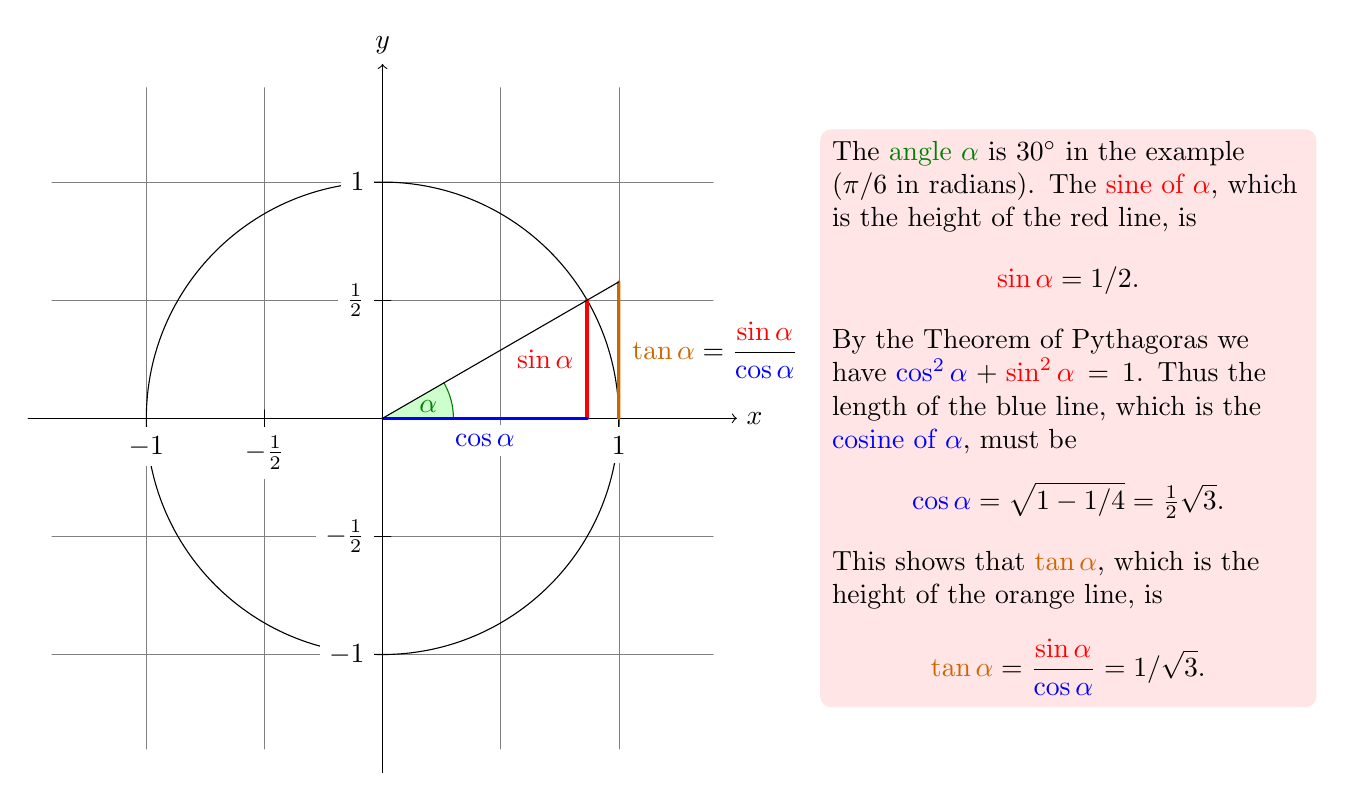
\begin{tikzpicture}
  [scale=3,line cap=round,
   % Styles
   axes/.style=,
   important line/.style={very thick},
   information text/.style={rounded corners,fill=red!10,inner sep=1ex}]

  % Local definitions
  \def\costhirty{0.8660256}

  % Colors
  \colorlet{anglecolor}{green!50!black}
  \colorlet{sincolor}{red}
  \colorlet{tancolor}{orange!80!black}
  \colorlet{coscolor}{blue}

  % The graphic
  \draw[help lines,step=0.5cm] (-1.4,-1.4) grid (1.4,1.4);

  \draw (0,0) circle [radius=1cm];

  \begin{scope}[axes]
    \draw[->] (-1.5,0) -- (1.5,0) node[right] {$x$};
    \draw[->] (0,-1.5) -- (0,1.5) node[above] {$y$};

    \foreach \x/\xtext in {-1, -.5/-\frac{1}{2}, 1}
      \draw[xshift=\x cm] (0pt,1pt) -- (0pt,-1pt) node[below,fill=white] {$\xtext$};

    \foreach \y/\ytext in {-1, -.5/-\frac{1}{2}, .5/\frac{1}{2}, 1}
      \draw[yshift=\y cm] (1pt,0pt) -- (-1pt,0pt) node[left,fill=white] {$\ytext$};
  \end{scope}

  \filldraw[fill=green!20,draw=anglecolor] (0,0) -- (3mm,0pt) arc(0:30:3mm);
  \draw (15:2mm) node[anglecolor] {$\alpha$};

  \draw[important line,sincolor]
    (30:1cm) -- node[left=1pt,fill=white] {$\sin \alpha$} +(0,-.5);

  \draw[important line,coscolor]
    (0,0) -- node[below=2pt,fill=white] {$\cos \alpha$} (\costhirty,0);

  \draw[important line,tancolor] (1,0) --
    node [right=1pt,fill=white]
    {
      $\displaystyle \tan \alpha \color{black}=
      \frac{{\color{sincolor}\sin \alpha}}{\color{coscolor}\cos \alpha}$
    } (intersection of 0,0--30:1cm and 1,0--1,1) coordinate (t);

  \draw (0,0) -- (t);

  \draw[xshift=1.85cm] node [right,text width=6cm,information text]
    {
      The {\color{anglecolor} angle $\alpha$} is $30^\circ$ in the
      example ($\pi/6$ in radians). The {\color{sincolor}sine of
        $\alpha$}, which is the height of the red line, is
      \[
      {\color{sincolor} \sin \alpha} = 1/2.
      \]
      By the Theorem of Pythagoras we have ${\color{coscolor}\cos^2 \alpha} +
      {\color{sincolor}\sin^2\alpha} =1$. Thus the length of the blue
      line, which is the {\color{coscolor}cosine of $\alpha$}, must be
      \[
      {\color{coscolor}\cos\alpha} = \sqrt{1 - 1/4} = \textstyle
      \frac{1}{2} \sqrt 3.
      \]%
      This shows that {\color{tancolor}$\tan \alpha$}, which is the
      height of the orange line, is
      \[
      {\color{tancolor}\tan\alpha} = \frac{{\color{sincolor}\sin
          \alpha}}{\color{coscolor}\cos \alpha} = 1/\sqrt 3.
      \]%
    };
\end{tikzpicture}
% \end{flushright}
\switchcolumn
\noindent
\begin{tikzpicture}%用于创建TikZ图形的代码。
  [scale=3,line cap=round,
   % Styles 定义了一些自定义样式,可以在整个图形中使用。
   axes/.style=,
   important line/.style={very thick},
   information text/.style={rounded corners,fill=red!10,inner sep=1ex}]

  % Local definitions 
  \def\costhirty{0.8660256}

  % Colors
  \colorlet{anglecolor}{green!50!black}
  \colorlet{sincolor}{red}
  \colorlet{tancolor}{orange!80!black}
  \colorlet{coscolor}{blue}

  % The graphic 绘制了一个网格,使用了帮助线样式,并且每0.5cm有一条线。
  \draw[help lines,step=0.5cm] (-1.4,-1.4) grid (1.4,1.4);

  \draw (0,0) circle [radius=1cm];%绘制了一个以原点(0,0)为中心,半径为1cm的圆。

  \begin{scope}[axes]
    \draw[->] (-1.5,0) -- (1.5,0) node[right] {$x$轴};
    \draw[->] (0,-1.5) -- (0,1.5) node[above] {$y$轴};%绘制了x和y坐标轴。

    \foreach \x/\xtext in {-1, -.5/-\frac{1}{2}, 1}
      \draw[xshift=\x cm] (0pt,1pt) -- (0pt,-1pt) node[below,fill=white] {$\xtext$};

    \foreach \y/\ytext in {-1, -.5/-\frac{1}{2}, .5/\frac{1}{2}, 1}
      \draw[yshift=\y cm] (1pt,0pt) -- (-1pt,0pt) node[left,fill=white] {$\ytext$};
      % \x/\xtext 和 \y/\ytext 是 \foreach 循环中使用的变量。
      % \x 和 \y 是循环的当前值,\xtext 和 \ytext 是对应的标签文本。
      % 如果只提供了一个值(如 -1),则 \xtext 或 \ytext 会被设置为相同的值。
      % 如果提供了两个值(如 -.5/-\frac{1}{2}),第一个是 \x 或 \y 的值,第二个是 \xtext 或 \ytext 的值。
  \end{scope}

  \filldraw[fill=green!20,draw=anglecolor] (0,0) -- (3mm,0pt) arc(0:30:3mm);%绘制了一个表示角度α的弧,并用绿色填充了它。
  \draw (15:2mm) node[anglecolor] {$\alpha$};%绘制一个点,并在该点的位置上标记角度符号α。

  \draw[important line,sincolor]
    (30:1cm) -- node[left=1pt,fill=white] {$\sin \alpha$} +(0,-.5);%绘制一条从原点开始的线段,表示正弦函数的值。这条线段位于角度α的位置,长度为1cm,并且标有$\sin \alpha$的标签。

  \draw[important line,coscolor]
    (0,0) -- node[below=2pt,fill=white] {$\cos \alpha$} (\costhirty,0);%绘制一条水平线段,表示余弦函数的值。这条线段的长度为$\cos 30^\circ$,并且标有$\cos \alpha$的标签。

  %绘制一条从点(1,0)开始的线段,表示正切函数的值。这条线段的斜率等于$\frac{{\sin \alpha}}{{\cos \alpha}}$,并且标有$\tan \alpha$的标签。该线段与前面绘制的两条线段相交,交点的坐标被命名为(t)。
  \draw[important line,tancolor] (1,0) --
    node [right=1pt,fill=white]
    {
      $\displaystyle \tan \alpha \color{black}=
      \frac{{\color{sincolor}\sin \alpha}}{\color{coscolor}\cos \alpha}$
    } (intersection of 0,0--30:1cm and 1,0--1,1) coordinate (t);

  \draw (0,0) -- (t);%绘制一条连接原点和点(t)的线段。

  %在指定的位置绘制一个文本框,用于提供关于三角函数图形的说明。文本框右侧有一条竖线,并包含了一些文本和数学公式。
  \draw[xshift=1.85cm] node [right,text width=6cm,information text]
    {      
      这个{\color{anglecolor} 角度 $\alpha$}在例子中是 $30^\circ$(弧度为 $\pi/6$)。{\color{sincolor} $\alpha$ 的正弦},也就是红线的高度,是

      \[
      {\color{sincolor} \sin \alpha} = 1/2.
      \]
     
      根据勾股定理,我们有 ${\color{coscolor}\cos^2 \alpha} +
      {\color{sincolor}\sin^2\alpha} =1$。因此,蓝线的长度,也就是{\color{coscolor} $\alpha$ 的余弦},必须是

      \[
      {\color{coscolor}\cos\alpha} = \sqrt{1 - 1/4} = \textstyle
      \frac{1}{2} \sqrt 3.
      \]%

      这表明{\color{tancolor} $\alpha$ 的正切},也就是橙线的高度,是
      \[
      {\color{tancolor}\tan\alpha} = \frac{{\color{sincolor}\sin
          \alpha}}{\color{coscolor}\cos \alpha} = 1/\sqrt 3.
      \]%
    };
\end{tikzpicture}

\switchcolumn[0]*
\subsection{Setting up the Environment}
\switchcolumn
\subsection{Setting up the Environment\\设置环境}
\switchcolumn[0]*
In \tikzname, to draw a picture, at the start of the picture you need to tell
\TeX\ or \LaTeX\ that you want to start a picture. In \LaTeX\ this is done
using the environment |{tikzpicture}|, in plain \TeX\ you just use
|\tikzpicture| to start the picture and |\endtikzpicture| to end it.
\switchcolumn
在\tikzname 中,要绘制一个图形,你需要在图形开始时告诉\TeX\ 或\LaTeX\ 你想要开始一个图形。在\LaTeX\ 中,使用环境 |{tikzpicture}| 来完成这个操作,在plain \TeX\ 中,你只需使用 |\tikzpicture| 来开始图形,使用 |\endtikzpicture| 来结束图形。
\switchcolumn[0]*
\subsubsection{Setting up the Environment in \LaTeX}
\switchcolumn
\subsubsection{在 \LaTeX 中设置环境}
\switchcolumn[0]*
Karl, being a \LaTeX\ user, thus sets up his file as follows:
%
\switchcolumn
作为一个 \LaTeX 用户,Karl 设置他的文件如下:
\switchcolumn[0]*
\begin{codeexample}[code only]
\documentclass{article} % say
\usepackage{tikz}
\begin{document}
We are working on
\begin{tikzpicture}
  \draw (-1.5,0) -- (1.5,0);
  \draw (0,-1.5) -- (0,1.5);
\end{tikzpicture}.
\end{document}
\end{codeexample}
\switchcolumn
\begin{codeexample}[code only]
\documentclass{article} % say
\usepackage{tikz}
\begin{document}
We are working on
\begin{tikzpicture}
  \draw (-1.5,0) -- (1.5,0);
  \draw (0,-1.5) -- (0,1.5);
\end{tikzpicture}.
\end{document}
\end{codeexample}
\switchcolumn[0]*
When executed, that is, run via |pdflatex| or via |latex| followed by |dvips|,
the resulting will contain something that looks like this:
\switchcolumn
当执行该代码,即通过 |pdflatex| 或 |latex| 后跟 |dvips| 运行时,结果将会包含以下内容:
\switchcolumn[0]*
\begin{dispExample*}{sidebyside}
We are working on
\begin{tikzpicture}
  \draw (-1.5,0) -- (1.5,0);
  \draw (0,-1.5) -- (0,1.5);
\end{tikzpicture}.
\end{dispExample*}
\switchcolumn
\begin{dispExample*}{sidebyside}
我们正在绘制
\begin{tikzpicture}
  \draw (-1.5,0) -- (1.5,0); % 绘制一条横轴
  \draw (0,-1.5) -- (0,1.5); % 绘制一条纵轴
\end{tikzpicture}。
\end{dispExample*}

% \begin{codeexample}[width=7cm]
% We are working on
% \begin{tikzpicture}
%   \draw (-1.5,0) -- (1.5,0);
%   \draw (0,-1.5) -- (0,1.5);
% \end{tikzpicture}.
% \end{codeexample}

\switchcolumn[0]*
Admittedly, not quite the whole picture, yet, but we do have the axes
established. Well, not quite, but we have the lines that make up the axes
drawn. Karl suddenly has a sinking feeling that the picture is still some way
off.
\switchcolumn
诚然,这还不是完整的图像,但我们已经建立了坐标轴。嗯,并不完全准确,但我们已经绘制了构成坐标轴的线段。Karl 突然有一种不安的感觉,认为图像还有一段路要走。
\switchcolumn[0]*
Let's have a more detailed look at the code. First, the package |tikz| is
loaded. This package is a so-called ``frontend'' to the basic \pgfname\ system.
The basic layer, which is also described in this manual, is somewhat more,
well, basic and thus harder to use. The frontend makes things easier by
providing a simpler syntax.
\switchcolumn
让我们更详细地看一下代码。首先,加载了 |tikz| 宏包。该宏包是基本 \pgfname\ 系统的所谓“前端”。基本层在本手册中也有所描述,它更基础一些,因此使用起来更困难。前端通过提供更简单的语法使事情更容易。
\switchcolumn[0]*
Inside the environment there are two |\draw| commands. They mean: ``The path,
which is specified following the command up to the semicolon, should be
drawn.'' The first path is specified as |(-1.5,0) -- (0,1.5)|, which means ``a
straight line from the point at position $(-1.5,0)$ to the point at position
$(0,1.5)$''. Here, the positions are specified within a special coordinate
system in which, initially, one unit is 1cm.
\switchcolumn
在环境内部有两个 |\draw| 命令。它们的意思是:“应该绘制路径,路径在命令后面到分号之前指定。”第一个路径被指定为 |(-1.5,0) -- (0,1.5)|,意思是“从位置 $(-1.5,0)$ 到位置 $(0,1.5)$ 绘制一条直线”。这里,位置在一个特殊的坐标系中指定,初始情况下,一个单位等于 1cm。
\switchcolumn[0]*
Karl is quite pleased to note that the environment automatically reserves
enough space to encompass the picture.
\switchcolumn
Karl 很高兴地注意到环境会自动保留足够的空间来容纳图片。

\switchcolumn[0]*
\subsubsection{Setting up the Environment in Plain \TeX}
\switchcolumn
\subsubsection{在 Plain \TeX 中设置环境}

\switchcolumn[0]*
Karl's wife Gerda, who also happens to be a math teacher, is not a \LaTeX\
user, but uses plain \TeX\ since she prefers to do things ``the old way''. She
can also use \tikzname. Instead of |\usepackage{tikz}| she has to write
|\input tikz.tex| and instead of |\begin{tikzpicture}| she writes
|\tikzpicture| and instead of |\end{tikzpicture}| she writes |\endtikzpicture|.
\switchcolumn
Karl 的妻子 Gerda 也是一名数学教师,她不使用 \LaTeX,而是使用 Plain \TeX,因为她更喜欢“老派”的方式。她也可以使用 \tikzname。她需要将 |\usepackage{tikz}| 替换为 |\input tikz.tex|,将 |\begin{tikzpicture}| 替换为 |\tikzpicture|,将 |\end{tikzpicture}| 替换为 |\endtikzpicture|。
\switchcolumn[0]*
Thus, she would use:
\switchcolumn
因此,她将使用以下代码:
\switchcolumn[0]*
\begin{codeexample}[code only]
%% Plain TeX file
\input tikz.tex
\baselineskip=12pt
\hsize=6.3truein
\vsize=8.7truein
We are working on
\tikzpicture
  \draw (-1.5,0) -- (1.5,0);
  \draw (0,-1.5) -- (0,1.5);
\endtikzpicture.
\bye
\end{codeexample}
\switchcolumn
\begin{codeexample}[code only]
%% Plain TeX file
\input tikz.tex
\baselineskip=12pt
\hsize=6.3truein
\vsize=8.7truein
我们正在绘制
\tikzpicture
  \draw (-1.5,0) -- (1.5,0);
  \draw (0,-1.5) -- (0,1.5);
\endtikzpicture.
\bye
\end{codeexample}

\switchcolumn[0]*
Gerda can typeset this file using either |pdftex| or |tex| together with
|dvips|. \tikzname\ will automatically discern which driver she is using. If
she wishes to use |dvipdfm| together with |tex|, she either needs to modify the
file |pgf.cfg| or can write |\def\pgfsysdriver{pgfsys-dvipdfm.def}| somewhere
\emph{before} she inputs |tikz.tex| or |pgf.tex|.
\switchcolumn
Gerda 可以使用 |pdftex| 或 |tex| 与 |dvips| 来排版此文件。\tikzname 会自动判断她使用的是哪个驱动程序。如果她希望使用 |dvipdfm| 与 |tex| 一起使用,她需要修改文件 |pgf.cfg|,或者可以在输入 |tikz.tex| 或 |pgf.tex| 之前的某个地方写上 |\def\pgfsysdriver{pgfsys-dvipdfm.def}|。

\switchcolumn[0]*
\subsubsection{Setting up the Environment in Con\TeX t}
\switchcolumn
\subsubsection{在 Con\TeX t 中设置环境}
\switchcolumn[0]*
Karl's uncle Hans uses Con\TeX t. Like Gerda, Hans can also use \tikzname.
Instead of |\usepackage{tikz}| he says |\usemodule[tikz]|. Instead of
|\begin{tikzpicture}| he writes |\starttikzpicture| and  instead of
|\end{tikzpicture}| he writes |\stoptikzpicture|.
\switchcolumn
Karl 的叔叔 Hans 使用 Con\TeX t。和 Gerda 一样,Hans 也可以使用 \tikzname。他需要将 |\usepackage{tikz}| 替换为 |\usemodule[tikz]|。将 |\begin{tikzpicture}| 替换为 |\starttikzpicture|,将 |\end{tikzpicture}| 替换为 |\stoptikzpicture|。
\switchcolumn[0]*
His version of the example looks like this:
\switchcolumn
%
他的示例代码如下:
\switchcolumn[0]*
\begin{codeexample}[code only]
%% ConTeXt file
\usemodule[tikz]

\starttext
  We are working on
  \starttikzpicture
    \draw (-1.5,0) -- (1.5,0);
    \draw (0,-1.5) -- (0,1.5);
  \stoptikzpicture.
\stoptext
\end{codeexample}
\switchcolumn
\begin{codeexample}[code only]
%% ConTeXt file
\usemodule[tikz]

\starttext
我们正在绘制
  \starttikzpicture
    \draw (-1.5,0) -- (1.5,0);
    \draw (0,-1.5) -- (0,1.5);
  \stoptikzpicture.
\stoptext
\end{codeexample}

\switchcolumn[0]*
Hans will now typeset this file in the usual way using |texexec| or |context|.
\switchcolumn

Hans 可以使用 |texexec| 或 |context| 来排版这个文件。
\switchcolumn[0]*
\subsection{Straight Path Construction}
\switchcolumn
\subsection{直线路径构建}
\switchcolumn[0]*
The basic building block of all pictures in \tikzname\ is the path. A
\emph{path} is a series of straight lines and curves that are connected (that
is not the whole picture, but let us ignore the complications for the moment).
You start a path by specifying the coordinates of the start position as a point
in round brackets, as in |(0,0)|. This is followed by a series of ``path
extension operations''. The simplest is |--|, which we used already. It must be
followed by another coordinate and it extends the path in a straight line to
this new position. For example, if we were to turn the two paths of the axes
into one path, the following would result:
\switchcolumn
在\tikzname 中,所有图片的基本构建块是路径。一个\emph{路径}是由连接的直线和曲线组成的序列(这并不构成整个图片,但我们暂且忽略这些复杂性)。你可以通过将起始位置的坐标作为圆括号中的点来开始一个路径,例如 |(0,0)|。接下来是一系列的“路径扩展操作”。最简单的操作是 |--|,我们已经使用过了。它必须后跟另一个坐标,并将路径以直线延伸到新的位置。例如,如果我们将坐标轴的两条路径合并为一条路径,结果如下:
\switchcolumn[0]*
% \begin{codeexample}[]
% \tikz \draw (-1.5,0) -- (1.5,0) -- (0,-1.5) -- (0,1.5);
% \end{codeexample}
\begin{dispExample*}{sidebyside}
\tikz \draw (-1.5,0) -- (1.5,0) -- (0,-1.5) -- (0,1.5);
\end{dispExample*}
\switchcolumn
\begin{dispExample*}{sidebyside}
\tikz \draw (-1.5,0) -- (1.5,0) -- (0,-1.5) -- (0,1.5);
\end{dispExample*}

\switchcolumn[0]*
Karl is a bit confused by the fact that there is no |{tikzpicture}|
environment, here. Instead, the little command |\tikz| is used. This command
either takes one argument (starting with an opening brace as in
|\tikz{\draw (0,0) -- (1.5,0)}|, which yields \tikz{\draw (0,0) --(1.5,0);}) or
collects everything up to the next semicolon and puts it inside a
|{tikzpicture}| environment. As a rule of thumb, all \tikzname\ graphic drawing
commands must occur as an argument of |\tikz| or inside a |{tikzpicture}|
environment. Fortunately, the command |\draw| will only be defined inside this
environment, so there is little chance that you will accidentally do something
wrong here.
\switchcolumn
卡尔有点困惑,因为这里没有 |{tikzpicture}| 环境。取而代之,使用了命令 |\tikz|。这个命令可以接受一个参数(以打开的大括号开始,比如 |\tikz{\draw (0,0) -- (1.5,0)}|,它会生成 \tikz{\draw (0,0) --(1.5,0);})或者收集直到下一个分号的所有内容,并将其放入 |{tikzpicture}| 环境中。作为经验法则,所有的 \tikzname 图形绘制命令必须作为 |\tikz| 的参数或者在 |{tikzpicture}| 环境内部。幸运的是,命令 |\draw| 只会在此环境内部定义,所以你很少会在这里意外地做错事。

\switchcolumn[0]*
\subsection{Curved Path Construction}
\switchcolumn
\subsection{曲线路径构建}
\switchcolumn[0]*
The next thing Karl wants to do is to draw the circle. For this, straight lines
obviously will not do. Instead, we need some way to draw curves. For this,
\tikzname\ provides a special syntax. One or two ``control points'' are needed.
The math behind them is not quite trivial, but here is the basic idea: Suppose
you are at point $x$ and the first control point is $y$. Then the curve will
start ``going in the direction of~$y$ at~$x$'', that is, the tangent of the
curve at $x$ will point toward~$y$. Next, suppose the curve should end at $z$
and the second support point is $w$. Then the curve will, indeed, end at $z$
and the tangent of the curve at point $z$ will go through $w$.
\switchcolumn
卡尔接下来想要做的是绘制圆。显然,直线无法实现这一点。相反,我们需要一种方法来绘制曲线。为此,\tikzname 提供了一种特殊的语法。需要一个或两个“控制点”。它们背后的数学并不是非常复杂,但基本思想是:假设你在点 $x$,第一个控制点是 $y$。那么曲线将在“以 $x$ 为中心向 $y$ 的方向开始”,也就是说,曲线在点 $x$ 的切线将指向 $y$。接下来,假设曲线应该在 $z$ 结束,第二个支撑点是 $w$。那么曲线确实会在 $z$ 结束,并且曲线在点 $z$ 的切线将经过 $w$。
\switchcolumn[0]*
Here is an example (the control points have been added for clarity):
\switchcolumn
这是一个示例(为了清晰起见,添加了控制点):
\switchcolumn[0]*
% \begin{codeexample}[]
% \begin{tikzpicture}
%   \filldraw [gray] (0,0) circle [radius=2pt]
%                    (1,1) circle [radius=2pt]
%                    (2,1) circle [radius=2pt]
%                    (2,0) circle [radius=2pt];
%   \draw (0,0) .. controls (1,1) and (2,1) .. (2,0);
% \end{tikzpicture}
% \end{codeexample}
\begin{dispExample*}{sidebyside}
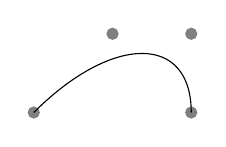
\begin{tikzpicture}
  \filldraw [gray] (0,0) circle [radius=2pt]
                   (1,1) circle [radius=2pt]
                   (2,1) circle [radius=2pt]
                   (2,0) circle [radius=2pt];
  \draw (0,0) .. controls (1,1) and (2,1) .. (2,0);
\end{tikzpicture}
\end{dispExample*}
\switchcolumn
\begin{dispExample*}{sidebyside}
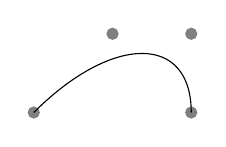
\begin{tikzpicture}
\filldraw [gray] (0,0) circle [radius=2pt]
                  (1,1) circle [radius=2pt]
                  (2,1) circle [radius=2pt]
                  (2,0) circle [radius=2pt];
\draw (0,0) .. controls (1,1) and (2,1) .. (2,0);
\end{tikzpicture}
\end{dispExample*}

\switchcolumn[0]*
The general syntax for extending a path in a ``curved'' way is |.. controls|
\meta{first control point} |and| \meta{second control point} |..|
\meta{end point}. You can leave out the |and| \meta{second control point},
which causes the first one to be used twice.
\switchcolumn
通过使用 |.. controls| \meta{第一个控制点} |and| \meta{第二个控制点} |..| \meta{结束点} 的一般语法,可以以“曲线”的方式扩展路径。可以省略 |and| \meta{第二个控制点},这样将使用第一个控制点两次。
\end{paracol}

%%% 以下gpt
在LaTeX中,这个命令是用于在TikZ库中绘制一条贝塞尔曲线。TikZ是一个非常强大的工具,用于创建矢量图形。 
\verb|\draw (0,0) .. controls (1,1) and (2,1) .. (2,0);| 这行代码的意思是从点 (0,0) 到点 (2,0) 绘制一条贝塞尔曲线,其中 (1,1) 和 (2,1) 是控制点。下面是对这个命令的详细解读:

\verb|\draw| 是 TikZ中的一个命令,它指示LaTeX开始绘制一条线或曲线。\verb|(0,0)| 是你要开始绘制的曲线的起始点,坐标是 (0,0)。\verb|.. controls (1,1) and (2,1) ..| 告诉LaTeX你要绘制的是一条贝塞尔曲线,而不是直线。关键词 controls 后面的两个点 (1,1) 和 (2,1) 是控制曲线形状的控制点。\verb|(2,0)| 是你要结束绘制的曲线的终点,坐标是 (2,0)。

贝塞尔曲线是一种数学曲线,用于描述平滑的曲线路径。它由数个控制点确定,通过这些控制点的位置和权重,可以定义曲线的形状。

贝塞尔曲线最常见的形式是二次贝塞尔曲线和三次贝塞尔曲线。二次贝塞尔曲线由三个控制点确定,分别为起始点、终点和一个中间点。三次贝塞尔曲线由四个控制点确定,分别为起始点、终点和两个中间点。

贝塞尔曲线的形状由控制点之间的插值算法确定。在二次贝塞尔曲线中,起始点和终点是曲线的端点,而中间点则会影响曲线的弯曲程度和方向。在三次贝塞尔曲线中,除了起始点和终点外,两个中间点的位置和权重也会影响曲线的形状。

贝塞尔曲线具有平滑性和局部控制性的特点。通过调整控制点的位置和权重,可以创建各种形状的曲线,包括弧线、圆弧、S形曲线等。贝塞尔曲线在计算机图形学、计算机辅助设计(CAD)、动画和游戏开发等领域得到广泛应用。

在绘图软件和绘图库中,如Adobe Illustrator、Inkscape和TikZ等,贝塞尔曲线通常由控制点和曲线类型(二次或三次)来定义。通过调整控制点的位置,可以实时预览和修改曲线的形状,从而满足具体的设计需求。

贝塞尔曲线具有以下几个特点:
通过移动控制点,可以方便地改变曲线的形状。
曲线必然通过第一个和最后一个控制点。
曲线在控制点附近的形状主要由相邻的几个控制点决定。
随着控制点数量的增加,贝塞尔曲线可以逼近任意形状。
贝塞尔曲线是可微的并且连续。
贝塞尔曲线计算简单,适合在计算机上实现。
贝塞尔曲线可以方便地进行仿射变换。
% 贝塞尔曲线在许多图形软件中都有应用,如Adobe Illustrator和Inkscape等。它为设计师提供了一个简单直观的方法来绘制平滑曲线。

贝塞尔曲线的应用:
贝塞尔曲线在计算机图形学中有着广泛的应用,例如用于绘制图形、生成动画等。
绘制图形:贝塞尔曲线可以用于绘制各种各样的图形,例如线条、曲线、图形等。
生成动画:贝塞尔曲线可以用于生成动画,例如人物动画、物体动画等。
图像处理:贝塞尔曲线可以用于图像处理,例如图像变形、图像合成等。

贝塞尔曲线具有以下优点:
光滑:贝塞尔曲线是光滑的,即曲线在任何点的切线都是连续的。
可变形:贝塞尔曲线可以通过控制点进行任意形状的变形。
通用性:贝塞尔曲线可以用来生成任意阶的多项式曲线。

贝塞尔曲线具有以下缺点:
计算复杂:贝塞尔曲线的计算比较复杂。
存储空间大:贝塞尔曲线的存储空间比较大。

%%% gpt结束 

\columnratio{0.55}
\begin{paracol}{2}
\switchcolumn[0]*
So, Karl can now add the first half circle to the picture:
\switchcolumn
因此,卡尔现在可以将第一个半圆添加到图片中:
\switchcolumn[0]*
\begin{dispExample*}{sidebyside}
\begin{tikzpicture}
  \draw (-1.5,0) -- (1.5,0);
  \draw (0,-1.5) -- (0,1.5);
  \draw (-1,0) .. controls (-1,0.555) and (-0.555,1) .. (0,1)
               .. controls (0.555,1) and (1,0.555) .. (1,0);
\end{tikzpicture}
\end{dispExample*}
\switchcolumn
\begin{dispExample*}{sidebyside}
\begin{tikzpicture}
  \draw (-1.5,0) -- (1.5,0);
  \draw (0,-1.5) -- (0,1.5);
  \draw (-1,0) .. controls (-1,0.555) and (-0.555,1) .. (0,1)
               .. controls (0.555,1) and (1,0.555) .. (1,0);
\end{tikzpicture}
\end{dispExample*}


% \begin{codeexample}[]
% % \begin{tikzpicture}
% %   \draw (-1.5,0) -- (1.5,0);
% %   \draw (0,-1.5) -- (0,1.5);
% %   \draw (-1,0) .. controls (-1,0.555) and (-0.555,1) .. (0,1)
% %                .. controls (0.555,1) and (1,0.555) .. (1,0);
% % \end{tikzpicture}
% \end{codeexample}


\end{paracol}
%gpt
如果你想要计算出特定的控制点来绘制标准的圆形,通常将控制点设置在起点和终点沿切线方向的距离为圆半径的 $4(\sqrt{2}-1)/3 \approx 0.55228$ 倍的位置。这个值是通过解析法计算得出的,以确保贝塞尔曲线近似于圆弧。

对于一个圆形,通常使用四段三次贝塞尔曲线来近似绘制一个完整的圆。为了确保这些曲线近似于圆的形状,控制点必须精心选择。

三次贝塞尔曲线由四个点定义:起点 $P_0$、两个控制点 $P_1$ 和 $P_2$、以及终点 $P_3$。曲线形状由这些点通过以下参数方程描述:
\[
B(t) = (1-t)^3 P_0 + 3(1-t)^2 t P_1 + 3(1-t) t^2 P_2 + t^3 P_3, \quad \text{其中} \quad t \in [0, 1]
\]

对于一个单位圆,我们可以将其分成四段,每段对应圆的一个象限。一种常见的做法是将起点和终点放在圆的四个八分点(即$0^\circ$、$90^\circ$、$180^\circ$、$270^\circ$)。控制点的选择是根据三次贝塞尔曲线与圆弧的相切性来确定的。

对于一个完整的圆,我们会将其分为四段,每段覆盖$90^\circ$。对于每段,起点和终点位于圆的正交方向上,比如第一段从$(1,0)$到$(0,1)$。控制点则位于起点和终点的切线方向上,距离为圆半径的$K$倍。

在数学上,$K$的值由以下等式给出:
\[
K = \frac{4}{3} \tan\left(\frac{\pi}{2n}\right)
\]
其中,$n$是曲线段的数量,对于圆来说是4(因为我们使用四段曲线)。因此我们有:
\[
K \approx \frac{4}{3} \tan\left(\frac{\pi}{8}\right) \approx 0.5522847498
\]

现在,以第一段为例,起点是 $(1,0)$(在单位圆的$0^\circ$处),终点是 $(0,1)$(在$90^\circ$处)。如果我们要从$(1,0)$开始绘制,第一个控制点 $P_1$ 将沿着起点的切线方向(向上)距离为$K$,即 $(1,K)$。第二个控制点 $P_2$ 将沿着终点的切线方向(向左)距离也为$K$,即 $(K,1)$。类似地,你可以为圆上的其他三段计算控制点。

因此,对于单位圆上从$(1,0)$到$(0,1)$的第一段,三次贝塞尔曲线的控制点是:
\[
P_1 = (1, K) = (1, 0.5522847498)
\]
\[
P_2 = (K, 1) = (0.5522847498, 1)
\]

使用这些控制点,我们可以绘制一个非常接近圆弧的三次贝塞尔曲线。对于其他三段也是以类似的方式确定控制点。注意控制点的位置相对于起点和终点的切线方向和距离是关键。

\columnratio{0.55}
\begin{paracol}{2}



\switchcolumn[0]*
Karl is happy with the result, but finds specifying circles in this way to be
extremely awkward. Fortunately, there is a much simpler way.
\switchcolumn
Karl对结果感到满意,但他发现用这种方式指定圆非常麻烦。幸运的是,有一种更简单的方法。
\switchcolumn[0]*
\subsection{Circle Path Construction}
\switchcolumn
\subsection{绘制圆形路径}

\switchcolumn[0]*
In order to draw a circle, the path construction operation |circle| can be
used. This operation is followed by a radius in brackets as in the following
example: (Note that the previous position is used as the \emph{center} of the
circle.)
\switchcolumn
为了绘制一个圆,可以使用路径构造操作|circle|。该操作后跟在括号内的半径,如下面的示例所示:(请注意,前一个位置被用作圆的\emph{中心}。)
\switchcolumn[0]*
% \begin{codeexample}[]
% \tikz \draw (0,0) circle [radius=10pt];
% \end{codeexample}
\begin{dispExample*}{sidebyside}
\tikz \draw (0,0) circle [radius=10pt];
\end{dispExample*}
\switchcolumn
\begin{dispExample*}{sidebyside}
\tikz \draw (0,0) circle [radius=10pt];
\end{dispExample*}
\switchcolumn[0]*
You can also append an ellipse to the path using the |ellipse| operation.
Instead of a single radius you can specify two of them:
\switchcolumn
您还可以使用|ellipse|操作将椭圆附加到路径上。您可以指定两个半径,而不是一个:
\switchcolumn[0]*
% \begin{codeexample}[]
% \tikz \draw (0,0) ellipse [x radius=20pt, y radius=10pt];
% \end{codeexample}
\begin{dispExample*}{sidebyside}
\tikz \draw (0,0) ellipse [x radius=20pt, y radius=10pt];
\end{dispExample*}
\switchcolumn
\begin{dispExample*}{sidebyside}
\tikz \draw (0,0) ellipse [x radius=20pt, y radius=10pt];
\end{dispExample*}
\switchcolumn[0]*
To draw an ellipse whose axes are not horizontal and vertical, but point in an
arbitrary direction (a ``turned ellipse'' like \tikz \draw[rotate=30] (0,0)
ellipse [x radius=6pt, y radius=3pt];) you can use transformations, which are
explained later. The code for the little ellipse is\\
|\tikz \draw[rotate=30] (0,0) ellipse [x radius=6pt, y radius=3pt];|, by the
way.
\switchcolumn
要绘制一个轴不是水平和垂直的椭圆,而是指向任意方向的椭圆(一个``旋转椭圆'',如\tikz \draw[rotate=30] (0,0) ellipse [x radius=6pt, y radius=3pt];),您可以使用后面将解释的变换。顺便说一下,小椭圆的代码是\\|\tikz \draw[rotate=30] (0,0) ellipse [x radius=6pt, y radius=3pt];|。
\switchcolumn[0]*
So, returning to Karl's problem, he can write
|\draw (0,0) circle [radius=1cm];| to draw the circle:
\switchcolumn
因此,回到Karl的问题,他可以写|\draw (0,0) circle [radius=1cm];|来绘制圆:
\switchcolumn[0]*
\begin{dispExample*}{sidebyside}
\begin{tikzpicture}
  \draw (-1.5,0) -- (1.5,0);
  \draw (0,-1.5) -- (0,1.5);
  \draw (0,0) circle [radius=1cm];
\end{tikzpicture}
\end{dispExample*}
\switchcolumn
\begin{dispExample*}{sidebyside}
\begin{tikzpicture}
  \draw (-1.5,0) -- (1.5,0);
  \draw (0,-1.5) -- (0,1.5);
  \draw (0,0) circle [radius=1cm];
\end{tikzpicture}
\end{dispExample*}

% \begin{codeexample}[]
% % \begin{tikzpicture}
% %   \draw (-1.5,0) -- (1.5,0);
% %   \draw (0,-1.5) -- (0,1.5);
% %   \draw (0,0) circle [radius=1cm];
% % \end{tikzpicture}
% \end{codeexample}
\switchcolumn[0]*
At this point, Karl is a bit alarmed that the circle is so small when he wants
the final picture to be much bigger. He is pleased to learn that \tikzname\ has
powerful transformation options and scaling everything by a factor of three is
very easy. But let us leave the size as it is for the moment to save some
space.
\switchcolumn
此时,Karl有点担心当他希望最终的图片更大时,圆太小了。他很高兴地知道\tikzname\ 有强大的变换选项,将所有内容放大三倍非常容易。但为了节省空间,让我们暂时保持尺寸不变。
\switchcolumn[0]*
\subsection{Rectangle Path Construction}
\switchcolumn
\subsection{矩形路径构造}
\switchcolumn[0]*
The next things we would like to have is the grid in the background. There are
several ways to produce it. For example, one might draw lots of rectangles.
Since rectangles are so common, there is a special syntax for them: To add a
rectangle to the current path, use the |rectangle| path construction operation.
This operation should be followed by another coordinate and will append a
rectangle to the path such that the previous coordinate and the next
coordinates are corners of the rectangle. So, let us add two rectangles to the
picture:
\switchcolumn
接下来我们想要的是背景中的网格。有几种方法可以实现。例如,可以绘制许多矩形。由于矩形非常常见,因此有一种特殊的语法可以用于绘制矩形:要将矩形添加到当前路径中,请使用|rectangle|路径构造操作。此操作后应跟另一个坐标,并将矩形附加到路径中,以使前一个坐标和下一个坐标成为矩形的角。让我们在图片中添加两个矩形:
\switchcolumn[0]*
\begin{dispExample*}{sidebyside}
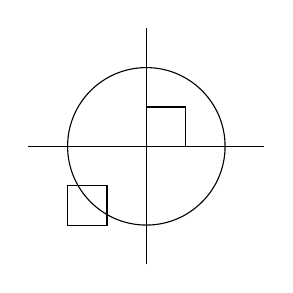
\begin{tikzpicture}
  \draw (-1.5,0) -- (1.5,0);
  \draw (0,-1.5) -- (0,1.5);
  \draw (0,0) circle [radius=1cm];
  \draw (0,0) rectangle (0.5,0.5);
  \draw (-0.5,-0.5) rectangle (-1,-1);
\end{tikzpicture}

\end{dispExample*}
\switchcolumn
\begin{dispExample*}{sidebyside}
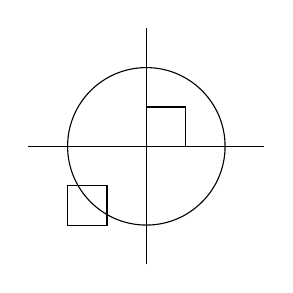
\begin{tikzpicture}
  \draw (-1.5,0) -- (1.5,0);
  \draw (0,-1.5) -- (0,1.5);
  \draw (0,0) circle [radius=1cm];
  \draw (0,0) rectangle (0.5,0.5);
  \draw (-0.5,-0.5) rectangle (-1,-1);
\end{tikzpicture}

\end{dispExample*}


\switchcolumn[0]*
While this may be nice in other situations, this is not really leading anywhere
with Karl's problem: First, we would need an awful lot of these rectangles and
then there is the border that is not ``closed''.
\switchcolumn
虽然在其他情况下这可能很好,但对于Karl的问题来说,这并没有真正解决问题:首先,我们需要大量这些矩形,其次边界并没有被“闭合”。
\switchcolumn[0]*
So, Karl is about to resort to simply drawing four vertical and four horizontal
lines using the nice |\draw| command, when he learns that there is a |grid|
path construction operation.
\switchcolumn
所以,当Karl打算使用简单的|\draw|命令绘制四条垂直线和四条水平线时,他得知有一个|grid|路径构造操作。

\switchcolumn[0]*
\subsection{Grid Path Construction}
\switchcolumn
\subsection{网格路径构造}
\switchcolumn[0]*
The |grid| path operation adds a grid to the current path. It will add lines
making up a grid that fills the rectangle whose one corner is the current point
and whose other corner is the point following the |grid| operation. For
example, the code |\tikz \draw[step=2pt] (0,0) grid (10pt,10pt);| produces
\tikz \draw[step=2pt] (0,0) grid (10pt,10pt);. Note how the optional argument
for |\draw| can be used to specify a grid width (there are also |xstep| and
|ystep| to define the steppings independently). As Karl will learn soon, there
are \emph{lots} of things that can be influenced using such options.
\switchcolumn
|grid|路径操作将网格添加到当前路径中。它将添加构成填充由当前点和|grid|操作后的点确定的矩形的网格线。例如,代码|\tikz \draw[step=2pt] (0,0) grid (10pt,10pt);|将产生\tikz \draw[step=2pt] (0,0) grid (10pt,10pt);。请注意,|\draw|的可选参数可用于指定网格宽度(也有|xstep|和|ystep|可单独定义步进)。正如Karl很快会了解到的,有很多事情可以通过这些选项来控制。
\switchcolumn[0]*
For Karl, the following code could be used:
\switchcolumn
对于Karl来说,可以使用以下代码:
\switchcolumn[0]*
\begin{dispExample*}{sidebyside}
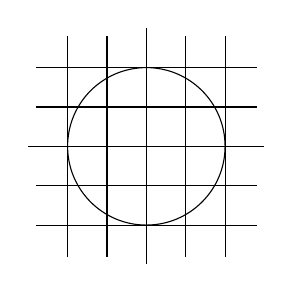
\begin{tikzpicture}
  \draw (-1.5,0) -- (1.5,0);
  \draw (0,-1.5) -- (0,1.5);
  \draw (0,0) circle [radius=1cm];
  \draw[step=.5cm] (-1.4,-1.4) grid (1.4,1.4);
\end{tikzpicture}

\end{dispExample*}
\switchcolumn
\begin{dispExample*}{sidebyside}
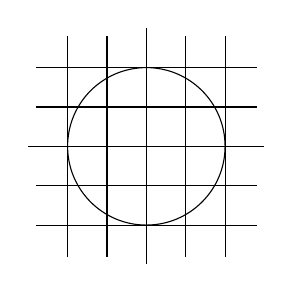
\begin{tikzpicture}
  \draw (-1.5,0) -- (1.5,0);
  \draw (0,-1.5) -- (0,1.5);
  \draw (0,0) circle [radius=1cm];
  \draw[step=.5cm] (-1.4,-1.4) grid (1.4,1.4);
\end{tikzpicture}

\end{dispExample*}

\switchcolumn[0]*
Having another look at the desired picture, Karl notices that it would be nice
for the grid to be more subdued. (His son told him that grids tend to be
distracting if they are not subdued.) To subdue the grid, Karl adds two more
options to the |\draw| command that draws the grid. First, he uses the color
|gray| for the grid lines. Second, he reduces the line width to |very thin|.
Finally, he swaps the ordering of the commands so that the grid is drawn first
and everything else on top.
\switchcolumn
再次查看所需的图片,Karl注意到网格更加柔和会更好(他的儿子告诉他,如果网格没有柔和处理,会分散注意力)。为了使网格柔和,Karl向绘制网格的|\draw|命令添加了两个选项。首先,他使用|gray|颜色绘制网格线。其次,他将线宽减小为|very thin|。最后,他交换了命令的顺序,使网格先绘制,其他内容在其上绘制。
\switchcolumn[0]*
\begin{dispExample*}{sidebyside}
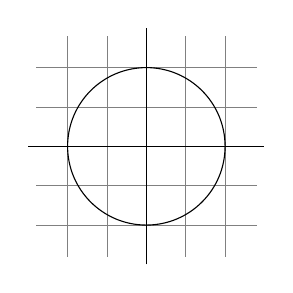
\begin{tikzpicture}
  \draw[step=.5cm,gray,very thin] (-1.4,-1.4) grid (1.4,1.4);
  \draw (-1.5,0) -- (1.5,0);
  \draw (0,-1.5) -- (0,1.5);
  \draw (0,0) circle [radius=1cm];
\end{tikzpicture}

\end{dispExample*}
\switchcolumn
\begin{dispExample*}{sidebyside}
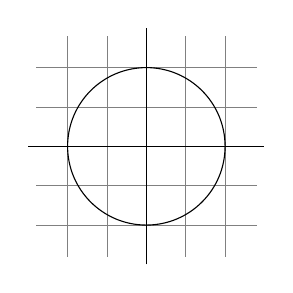
\begin{tikzpicture}
  \draw[step=.5cm,gray,very thin] (-1.4,-1.4) grid (1.4,1.4);
  \draw (-1.5,0) -- (1.5,0);
  \draw (0,-1.5) -- (0,1.5);
  \draw (0,0) circle [radius=1cm];
\end{tikzpicture}

\end{dispExample*}



\switchcolumn[0]*
\subsection{Adding a Touch of  Style}
\switchcolumn
\subsection{添加一点样式}
\switchcolumn[0]*
Instead of the options |gray,very thin| Karl could also have said |help lines|.
\emph{Styles} are predefined sets of options that can be used to organize how a
graphic is drawn. By saying |help lines| you say ``use the style that I (or
someone else) has set for drawing help lines''. If Karl decides, at some later
point, that grids should be drawn, say, using the color |blue!50| instead of
|gray|, he could provide the following option somewhere:
\switchcolumn
卡尔可以选择使用选项|gray,very thin|,也可以选择|help lines|。\emph{样式}是预定义的选项集,用于组织绘制图形的方式。通过使用|help lines|,你在实际上是在说“使用我(或其他人)为绘制辅助线设置的样式”。如果卡尔在以后的某个时间决定,网格应该使用颜色|blue!50|而不是|gray|来绘制,他可以在某个地方提供以下选项:
\switchcolumn[0]*
\begin{codeexample}[code only]
help lines/.style={color=blue!50,very thin}
\end{codeexample}
\switchcolumn[0]*
The effect of this ``style setter'' is that in the current scope or environment
the |help lines| option has the same effect as |color=blue!50,very thin|.
\switchcolumn
这个“样式设置器”的效果是,在当前的作用域或环境中,|help lines|选项具有与|color=blue!50,very thin|相同的效果。
\switchcolumn[0]*
Using styles makes your graphics code more flexible. You can change the way
things look easily in a consistent manner. Normally, styles are defined at the
beginning of a picture. However, you may sometimes wish to define a style
globally, so that all pictures of your document can use this style. Then you
can easily change the way all graphics look by changing this one style. In this
situation you can use the |\tikzset| command at the beginning of the document
as in
\switchcolumn
使用样式可以使你的图形代码更加灵活。你可以轻松以一致的方式改变事物的外观。通常,样式在图片的开头定义。然而,有时你可能希望全局定义一个样式,这样文档中的所有图片都可以使用这个样式。然后,你可以在文档开头使用|\tikzset|命令,如下所示:
\switchcolumn[0]*
\begin{codeexample}[code only]
\tikzset{help lines/.style=very thin}
\end{codeexample}
\switchcolumn[0]*
To build a hierarchy of styles you can have one style use another. So in order
to define a style |Karl's grid| that is based on the |grid| style Karl could
say
\switchcolumn
为了构建样式的层次结构,你可以让一个样式使用另一个样式。因此,为了定义一个基于样式|grid|的样式|Karl's grid|,卡尔可以这样说:
\switchcolumn[0]*
\begin{codeexample}[code only]
\tikzset{Karl's grid/.style={help lines,color=blue!50}}
...
\draw[Karl's grid] (0,0) grid (5,5);
\end{codeexample}
\switchcolumn[0]*
Styles are made even more powerful by parametrization. This means that, like
other options, styles can also be used with a parameter. For instance, Karl
could parameterize his grid so that, by default, it is blue, but he could also
use another color.
\switchcolumn
通过参数化,样式的功能更加强大。这意味着,像其他选项一样,样式也可以带有参数。例如,卡尔可以使他的网格参数化,以便默认情况下为蓝色,但他也可以使用其他颜色。
\switchcolumn[0]*
\begin{codeexample}[code only]
\begin{tikzpicture}
  [Karl's grid/.style  ={help lines,color=#1!50},
   Karl's grid/.default=blue]

  \draw[Karl's grid]     (0,0) grid (1.5,2);
  \draw[Karl's grid=red] (2,0) grid (3.5,2);
\end{tikzpicture}
\end{codeexample}
\switchcolumn[0]*
 In this example, the definition of the style |Karl's grid| is given as an
 optional argument to the |{tikzpicture}| environment. Additional styles for other
 elements would follow after a comma. With many styles in effect, the optional
 argument of the environment may easily happen to be longer than the actual
 contents.
\switchcolumn
 在这个例子中,样式|Karl's grid|的定义作为可选参数给出,放在|{tikzpicture}|环境中。其他元素的附加样式将在逗号后面跟随。当许多样式生效时,环境的可选参数可能比实际内容还要长。
\switchcolumn[0]*
\subsection{Drawing Options}
\switchcolumn
\subsection{绘制选项}
\switchcolumn[0]*
Karl wonders what other options there are that influence how a path is drawn.
He saw already that the |color=|\meta{color} option can be used to set the
line's color. The option |draw=|\meta{color} does nearly the same, only it sets
the color for the lines only and a different color can be used for filling
(Karl will need this when he fills the arc for the angle).
\switchcolumn
卡尔想知道还有哪些选项会影响路径的绘制方式。他已经看到了|color=|\meta{color}选项可以用于设置线条的颜色。选项|draw=|\meta{color}几乎相同,只是它只设置线条的颜色,可以使用不同的颜色进行填充(当卡尔填充角度的弧时会用到这个)。
\switchcolumn[0]*
He saw that the style |very thin| yields very thin lines. Karl is not really
surprised by this and neither is he surprised to learn that |thin| yields thin
lines,  |thick| yields thick lines, |very thick| yields very thick lines,
|ultra thick| yields really, really thick lines and |ultra thin| yields lines
that are so thin that low-resolution printers and displays will have trouble
showing them. He wonders what gives lines of ``normal'' thickness. It turns out
that |thin| is the correct choice, since it gives the same thickness as \TeX's
|\hrule| command. Nevertheless, Karl would like to know whether there is
anything ``in the middle'' between |thin| and |thick|. There is: |semithick|.
\switchcolumn
他已经看到 |very thin| 样式可以绘制非常细的线条。卡尔对此并不感到惊讶,他也不惊讶地了解到 |thin| 样式可以绘制细线条,|thick| 样式可以绘制粗线条,|very thick| 样式可以绘制非常粗的线条,|ultra thick| 样式可以绘制非常非常粗的线条,而 |ultra thin| 样式可以绘制非常细的线条,低分辨率的打印机和显示器可能无法显示它们。他想知道是否有一种线条厚度介于 |thin| 和 |thick| 之间的选项。答案是有的,这就是 |semithick|。
\switchcolumn[0]*
Another useful thing one can do with lines is to dash or dot them. For this,
the two styles |dashed| and |dotted| can be used, yielding \tikz[baseline]
\draw[dashed] (0,.5ex) -- ++(2em,0pt); and \tikz[baseline] \draw[dotted]
(0,.5ex) -- ++(2em,0pt);. Both options also exist in a loose and a dense
version, called |loosely dashed|, |densely dashed|, |loosely dotted|, and
|densely dotted|. If he really, really  needs to, Karl can also define much
more complex dashing patterns with the |dash pattern| option, but his son
insists that dashing is to be used with utmost care and mostly distracts.
Karl's son claims that complicated dashing patterns are evil. Karl's students
do not care about dashing patterns.
\switchcolumn
对于线条,还有一个有用的功能是虚线和点线。可以使用两个样式 |dashed| 和 |dotted|,分别绘制虚线和点线,得到的效果分别如下:\tikz[baseline] \draw[dashed] (0,.5ex) -- ++(2em,0pt); 和 \tikz[baseline] \draw[dotted] (0,.5ex) -- ++(2em,0pt);。这两个选项还有一种稀疏和稠密的版本,分别称为 |loosely dashed|、|densely dashed|、|loosely dotted| 和 |densely dotted|。如果卡尔确实需要的话,还可以使用 |dash pattern| 选项定义更复杂的虚线样式,但他的儿子坚持认为虚线应该小心使用,因为它们会分散注意力。卡尔的儿子声称复杂的虚线样式是有害的。卡尔的学生们对虚线样式不太关心。

\switchcolumn[0]*
\subsection{Arc Path Construction}
\switchcolumn
\subsection{弧路径构建}
\switchcolumn[0]*
Our next obstacle is to draw the arc for the angle. For this, the |arc| path
construction operation is useful, which draws part of a circle or ellipse. This
|arc| operation is followed by options in brackets that specify the arc. An
example would be \texttt{arc[start angle=10, end angle=80, radius=10pt]}, which
means exactly what it says. Karl obviously needs an arc from $0^\circ$ to
$30^\circ$. The radius should be something relatively small, perhaps around one
third of the circle's radius. When one uses the arc path construction
operation, the specified arc will be added with its starting point at the
current position. So, we first have to ``get there''.
\switchcolumn
下一个障碍是绘制角度的弧。为此,\texttt{arc}路径构建操作非常有用,它绘制了圆或椭圆的一部分。这个\texttt{arc}操作后面跟着方括号中指定弧的选项。一个例子是\texttt{arc[start angle=10, end angle=80, radius=10pt]},它的含义如字面意思所述。卡尔显然需要从$0^\circ$到$30^\circ$的弧。半径应该相对较小,可能是整个圆半径的三分之一左右。当使用弧路径构建操作时,指定的弧将从当前位置开始添加。因此,我们首先要“到达那里”。
\switchcolumn[0]*
\begin{dispExample*}{sidebyside}
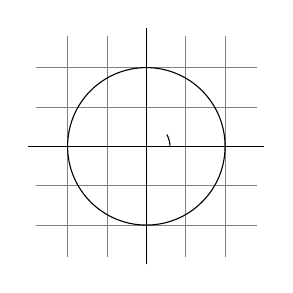
\begin{tikzpicture}
  \draw[step=.5cm,gray,very thin] (-1.4,-1.4) grid (1.4,1.4);
  \draw (-1.5,0) -- (1.5,0);
  \draw (0,-1.5) -- (0,1.5);
  \draw (0,0) circle [radius=1cm];
  \draw (3mm,0mm) arc [start angle=0, end angle=30, radius=3mm];
\end{tikzpicture}

\end{dispExample*}
\switchcolumn
\begin{dispExample*}{sidebyside}
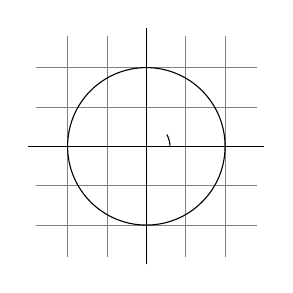
\begin{tikzpicture}
  \draw[step=.5cm,gray,very thin] (-1.4,-1.4) grid (1.4,1.4);
  \draw (-1.5,0) -- (1.5,0);
  \draw (0,-1.5) -- (0,1.5);
  \draw (0,0) circle [radius=1cm];
  \draw (3mm,0mm) arc [start angle=0, end angle=30, radius=3mm];
\end{tikzpicture}

\end{dispExample*}

\switchcolumn[0]*
Karl thinks this is really a bit small and he cannot continue unless he learns
how to do scaling. For this, he can add the |[scale=3]| option. He could add
this option to each |\draw| command, but that would be awkward. Instead, he
adds it to the whole environment, which causes this option to apply to
everything within.
\switchcolumn
卡尔认为这个弧太小了,除非他学会如何进行缩放,否则无法继续。为此,他可以添加\texttt{[scale=3]}选项。他可以将此选项添加到每个\texttt{\textbackslash draw}命令,但那样会很麻烦。相反,他将其添加到整个环境中,这使得此选项适用于其中的所有内容。
\switchcolumn[0]*
\begin{dispExample*}{sidebyside}
\begin{tikzpicture}[scale=3]
  \draw[step=.5cm,gray,very thin] (-1.4,-1.4) grid (1.4,1.4);
  \draw (-1.5,0) -- (1.5,0);
  \draw (0,-1.5) -- (0,1.5);
  \draw (0,0) circle [radius=1cm];
  \draw (3mm,0mm) arc [start angle=0, end angle=30, radius=3mm];
\end{tikzpicture}

\end{dispExample*}
\switchcolumn
\begin{dispExample*}{sidebyside}
\begin{tikzpicture}[scale=3]
  \draw[step=.5cm,gray,very thin] (-1.4,-1.4) grid (1.4,1.4);
  \draw (-1.5,0) -- (1.5,0);
  \draw (0,-1.5) -- (0,1.5);
  \draw (0,0) circle [radius=1cm];
  \draw (3mm,0mm) arc [start angle=0, end angle=30, radius=3mm];
\end{tikzpicture}

\end{dispExample*}

\switchcolumn[0]*
As for circles, you can specify ``two'' radii in order to get an elliptical
arc.
\switchcolumn
对于圆,您可以指定“两个”半径以得到椭圆弧。
\switchcolumn[0]*
\begin{dispExample*}{sidebyside}
  \tikz \draw (0,0)
    arc [start angle=0, end angle=315,
         x radius=1.75cm, y radius=1cm];

\end{dispExample*}
\switchcolumn
\begin{dispExample*}{sidebyside}
  \tikz \draw (0,0)
    arc [start angle=0, end angle=315,
         x radius=1.75cm, y radius=1cm];

\end{dispExample*}



\switchcolumn[0]*
\subsection{Clipping a Path}
\switchcolumn
\subsection{裁剪路径}
\switchcolumn[0]*
In order to save space in this manual, it would be nice to clip Karl's graphics
a bit so that we can focus on the ``interesting'' parts. Clipping is pretty
easy in \tikzname. You can use the |\clip| command to clip all subsequent
drawing. It works like |\draw|, only it does not draw anything, but uses the
given path to clip everything subsequently.
\switchcolumn
为了在本手册中节省空间,我们希望将卡尔的图形裁剪一下,以便我们可以专注于“有趣”的部分。在\tikzname 中,裁剪非常简单。您可以使用|\clip|命令来裁剪所有后续的绘图。它的使用方式类似于|\draw|,只是它不绘制任何东西,而是使用给定的路径来裁剪后续的一切。
\switchcolumn[0]*
\begin{dispExample*}{sidebyside}
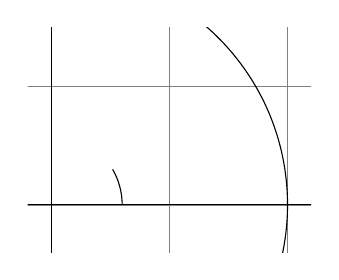
\begin{tikzpicture}[scale=3]
  \clip (-0.1,-0.2) rectangle (1.1,0.75);
  \draw[step=.5cm,gray,very thin] (-1.4,-1.4) grid (1.4,1.4);
  \draw (-1.5,0) -- (1.5,0);
  \draw (0,-1.5) -- (0,1.5);
  \draw (0,0) circle [radius=1cm];
  \draw (3mm,0mm) arc [start angle=0, end angle=30, radius=3mm];
\end{tikzpicture}

\end{dispExample*}
\switchcolumn
\begin{dispExample*}{sidebyside}
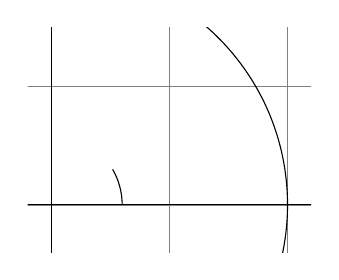
\begin{tikzpicture}[scale=3]
  \clip (-0.1,-0.2) rectangle (1.1,0.75);
  \draw[step=.5cm,gray,very thin] (-1.4,-1.4) grid (1.4,1.4);
  \draw (-1.5,0) -- (1.5,0);
  \draw (0,-1.5) -- (0,1.5);
  \draw (0,0) circle [radius=1cm];
  \draw (3mm,0mm) arc [start angle=0, end angle=30, radius=3mm];
\end{tikzpicture}

\end{dispExample*}


\switchcolumn[0]*
You can also do both at the same time: Draw \emph{and} clip a path. For this,
use the |\draw| command and add the |clip| option. (This is not the whole
picture: You can also use the |\clip| command and add the |draw| option. Well,
that is also not the whole picture: In reality, |\draw| is just a shorthand for
|\path[draw]| and |\clip| is a shorthand for |\path[clip]| and you could also
say |\path[draw,clip]|.) Here is an example:
\switchcolumn
您还可以同时绘制路径和剪裁路径。为此,请使用 |\draw| 命令并添加 |clip| 选项。(这还不是全部内容:您还可以使用 |\clip| 命令并添加 |draw| 选项。嗯,这还不是全部内容:实际上,|\draw| 只是 |\path[draw]| 的简写,|\clip| 是 |\path[clip]| 的简写,您也可以使用 |\path[draw,clip]|。)以下是一个示例:
\switchcolumn[0]*
\begin{dispExample*}{sidebyside}
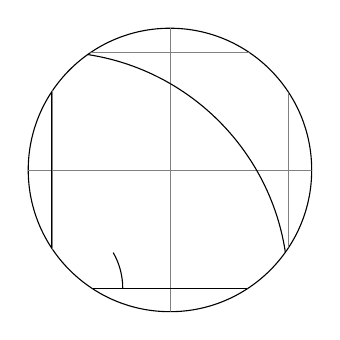
\begin{tikzpicture}[scale=3]
  \clip[draw] (0.5,0.5) circle (.6cm);
  \draw[step=.5cm,gray,very thin] (-1.4,-1.4) grid (1.4,1.4);
  \draw (-1.5,0) -- (1.5,0);
  \draw (0,-1.5) -- (0,1.5);
  \draw (0,0) circle [radius=1cm];
  \draw (3mm,0mm) arc [start angle=0, end angle=30, radius=3mm];
\end{tikzpicture}

\end{dispExample*}
\switchcolumn
\begin{dispExample*}{sidebyside}
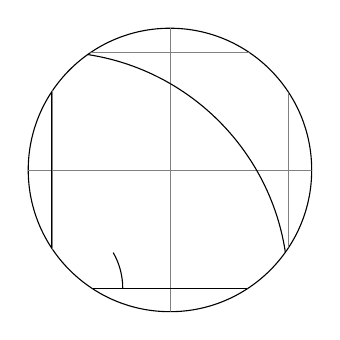
\begin{tikzpicture}[scale=3]
  \clip[draw] (0.5,0.5) circle (.6cm);
  \draw[step=.5cm,gray,very thin] (-1.4,-1.4) grid (1.4,1.4);
  \draw (-1.5,0) -- (1.5,0);
  \draw (0,-1.5) -- (0,1.5);
  \draw (0,0) circle [radius=1cm];
  \draw (3mm,0mm) arc [start angle=0, end angle=30, radius=3mm];
\end{tikzpicture}

\end{dispExample*}



\switchcolumn[0]*
\subsection{Parabola and Sine Path Construction}
\switchcolumn
\subsection{抛物线和正弦路径构造}

\switchcolumn[0]*
Although Karl does not need them for his picture, he is pleased to learn that
there are |parabola| and |sin| and |cos| path operations for adding parabolas
and sine and cosine curves to the current path. For the |parabola| operation,
the current point will lie on the parabola as well as the point given after the
parabola operation. Consider the following example:
\switchcolumn
虽然 Karl 并不需要它们来绘制他的图片,但他很高兴地了解到存在 |parabola|、|sin| 和 |cos| 路径操作,用于在当前路径中添加抛物线和正弦曲线以及余弦曲线。对于 |parabola| 操作,当前点将位于抛物线上,以及在抛物线操作之后给出的点上。考虑以下示例:
\switchcolumn[0]*
\begin{dispExample*}{sidebyside}
\tikz \draw (0,0) rectangle (1,1)  (0,0) parabola (1,1);

\end{dispExample*}
\switchcolumn
\begin{dispExample*}{sidebyside}
\tikz \draw (0,0) rectangle (1,1)  (0,0) parabola (1,1);

\end{dispExample*}

% (0,0) parabola (1,1) 这部分代码绘制了一条抛物线,起始点为 (0,0),终点为 (1,1)。抛物线经过起始点和终点,并且曲线形状由这两个点决定。
\switchcolumn[0]*
It is also possible to place the bend somewhere else:
\switchcolumn
也可以将曲线弯曲到其他位置:
\switchcolumn[0]*
\begin{dispExample*}{sidebyside}
\tikz \draw[x=1pt,y=1pt] (0,0) parabola bend (4,16) (6,12);

\end{dispExample*}
\switchcolumn
\begin{dispExample*}{sidebyside}
\tikz \draw[x=1pt,y=1pt] (0,0) parabola bend (4,16) (6,12);

\end{dispExample*}

%|(0,0) parabola bend (4,16) (6,12)|:这部分代码绘制了一条抛物线。起始点为 (0,0),通过 parabola 命令绘制的抛物线将起始点和终点 (4,16) 连接起来。然后,使用 bend 命令将曲线弯曲到另一个坐标点 (6,12)。
\switchcolumn[0]*
The operations |sin| and |cos| add a sine or cosine curve in the interval
$[0,\pi/2]$ such that the previous current point is at the start of the curve
and the curve ends at the given end point. Here are two examples:
\switchcolumn
|sin| 和 |cos| 操作在区间 $[0,\pi/2]$ 中添加正弦曲线或余弦曲线,使得前一个当前点位于曲线的起点,曲线在给定的终点结束。以下是两个示例:
\switchcolumn[0]*
\begin{dispExample*}{sidebyside}
A sine \tikz \draw[x=1ex,y=1ex] (0,0) sin (1.57,1); curve.

\end{dispExample*}
\switchcolumn
\begin{dispExample*}{sidebyside}
A sine \tikz \draw[x=1ex,y=1ex] (0,0) sin (1.57,1); curve.

\end{dispExample*}

% |x=1ex,y=1ex|:这部分代码设置了坐标系的缩放,将 x 和 y 方向的单位长度设置为 1ex。这样可以控制图形的尺寸。

% |(0,0) sin (1.57,1)|:这部分代码绘制了一条正弦曲线。起始点为 (0,0),通过 sin 命令绘制的曲线连接起始点和终点 (1.57,1)。

\begin{dispExample*}{sidebyside}
\tikz \draw[x=1.57ex,y=1ex] (0,0) sin (1,1) cos (2,0) sin (3,-1) cos (4,0)
                            (0,1) cos (1,0) sin (2,-1) cos (3,0) sin (4,1);

\end{dispExample*}
\switchcolumn
\begin{dispExample*}{sidebyside}
\tikz \draw[x=1.57ex,y=1ex] (0,0) sin (1,1) cos (2,0) sin (3,-1) cos (4,0)
                            (0,1) cos (1,0) sin (2,-1) cos (3,0) sin (4,1);

\end{dispExample*}


\switchcolumn[0]*
\subsection{Filling and Drawing}
\switchcolumn
\subsection{填充和绘制}
\switchcolumn[0]*
Returning to the picture, Karl now wants the angle to be ``filled'' with a very
light green. For this he uses |\fill| instead of |\draw|. Here is what Karl
does:
\switchcolumn
回到图形,Karl现在想要“填充”角度,使用非常浅的绿色。为此,他使用|\fill|而不是|\draw|。以下是Karl的操作:
\switchcolumn[0]*
\begin{dispExample*}{sidebyside}
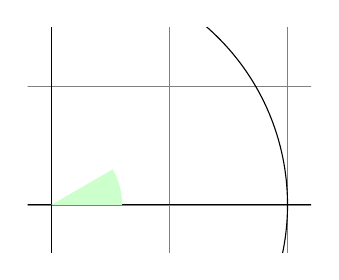
\begin{tikzpicture}[scale=3]
  \clip (-0.1,-0.2) rectangle (1.1,0.75);
  \draw[step=.5cm,gray,very thin] (-1.4,-1.4) grid (1.4,1.4);
  \draw (-1.5,0) -- (1.5,0);
  \draw (0,-1.5) -- (0,1.5);
  \draw (0,0) circle [radius=1cm];
  \fill[green!20!white] (0,0) -- (3mm,0mm)
    arc [start angle=0, end angle=30, radius=3mm] -- (0,0);
\end{tikzpicture}

\end{dispExample*}
\switchcolumn
\begin{dispExample*}{sidebyside}
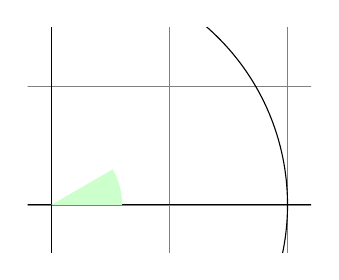
\begin{tikzpicture}[scale=3]
  \clip (-0.1,-0.2) rectangle (1.1,0.75);
  \draw[step=.5cm,gray,very thin] (-1.4,-1.4) grid (1.4,1.4);
  \draw (-1.5,0) -- (1.5,0);
  \draw (0,-1.5) -- (0,1.5);
  \draw (0,0) circle [radius=1cm];
  \fill[green!20!white] (0,0) -- (3mm,0mm)
    arc [start angle=0, end angle=30, radius=3mm] -- (0,0);
\end{tikzpicture}

\end{dispExample*}

% [green!20!white] 指定填充的颜色,是绿色和白色的混合,绿色占80%。
% (0,0) -- (3mm,0mm) 绘制一条线段,从(0,0)到(3mm,0mm)。
% arc 指定绘制一段圆弧。
% -- (0,0) 将终点和起点相连,形成封闭的路径。

\switchcolumn[0]*
The color |green!20!white| means 20\% green and 80\% white mixed together. Such
color expression are possible since \tikzname\ uses Uwe Kern's |xcolor|
package, see the documentation of that package for details on color
expressions.
\switchcolumn
颜色|green!20!white|表示20\%的绿色和80\%的白色混合在一起。由于\tikzname 使用了Uwe Kern的|xcolor|宏包,因此可以使用这种颜色表达式,请参阅该宏包的文档以了解有关颜色表达式的详细信息。
\switchcolumn[0]*
What would have happened, if Karl had not ``closed'' the path using |--(0,0)|
at the end? In this case, the path is closed automatically, so this could have
been omitted. Indeed, it would even have been better to write the following,
instead:
\switchcolumn
如果Karl在最后没有使用|--(0,0)|“闭合”路径会发生什么?在这种情况下,路径会自动闭合,因此可以省略这一部分。事实上,最好写成以下形式:
\switchcolumn[0]*
\begin{codeexample}[code only]
  \fill[green!20!white] (0,0) -- (3mm,0mm)
    arc [start angle=0, end angle=30, radius=3mm] -- cycle;
\end{codeexample}
\switchcolumn[0]*
The |--cycle| causes the current path to be closed (actually the current part
of the current path) by smoothly joining the first and last point. To
appreciate the difference, consider the following example:
\switchcolumn
|--cycle|通过平滑连接第一个和最后一个点来关闭当前路径(实际上是当前路径的当前部分)。为了体会到差异,请考虑以下示例:
\switchcolumn[0]*
\begin{dispExample*}{sidebyside}
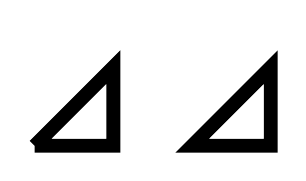
\begin{tikzpicture}[line width=5pt]
  \draw (0,0) -- (1,0) -- (1,1) -- (0,0);
  \draw (2,0) -- (3,0) -- (3,1) -- cycle;
  \useasboundingbox (0,1.5); % make bounding box higher
\end{tikzpicture}

\end{dispExample*}
\switchcolumn
\begin{dispExample*}{sidebyside}
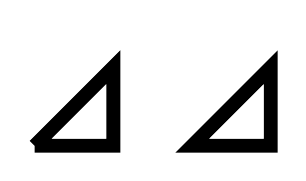
\begin{tikzpicture}[line width=5pt]
  \draw (0,0) -- (1,0) -- (1,1) -- (0,0);
  \draw (2,0) -- (3,0) -- (3,1) -- cycle;
  \useasboundingbox (0,1.5); % make bounding box higher
\end{tikzpicture}

\end{dispExample*}

\switchcolumn[0]*
You can also fill and draw a path at the same time using the |\filldraw|
command. This will first draw the path, then fill it. This may not seem too
useful, but you can specify different colors to be used for filling and for
stroking. These are specified as optional arguments like this:
\switchcolumn
你还可以同时填充和绘制路径,使用|\filldraw|命令。这将首先绘制路径,然后填充它。这可能看起来并不太有用,但是你可以指定用于填充和描边的不同颜色。这些颜色可以作为可选参数指定,如下所示:
\switchcolumn[0]*
\begin{dispExample*}{sidebyside}
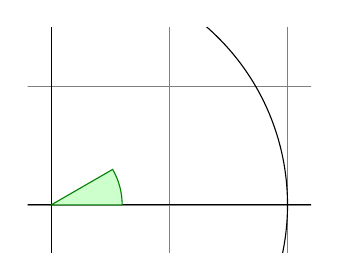
\begin{tikzpicture}[scale=3]
  \clip (-0.1,-0.2) rectangle (1.1,0.75);
  \draw[step=.5cm,gray,very thin] (-1.4,-1.4) grid (1.4,1.4);
  \draw (-1.5,0) -- (1.5,0);
  \draw (0,-1.5) -- (0,1.5);
  \draw (0,0) circle [radius=1cm];
  \filldraw[fill=green!20!white, draw=green!50!black] (0,0) -- (3mm,0mm)
    arc [start angle=0, end angle=30, radius=3mm] -- cycle;
\end{tikzpicture}

\end{dispExample*}
\switchcolumn
\begin{dispExample*}{sidebyside}
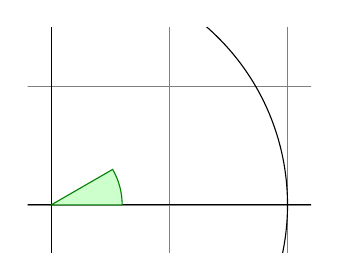
\begin{tikzpicture}[scale=3]
  \clip (-0.1,-0.2) rectangle (1.1,0.75);
  \draw[step=.5cm,gray,very thin] (-1.4,-1.4) grid (1.4,1.4);
  \draw (-1.5,0) -- (1.5,0);
  \draw (0,-1.5) -- (0,1.5);
  \draw (0,0) circle [radius=1cm];
  \filldraw[fill=green!20!white, draw=green!50!black] (0,0) -- (3mm,0mm)
    arc [start angle=0, end angle=30, radius=3mm] -- cycle;
\end{tikzpicture}

\end{dispExample*}



\switchcolumn[0]*
\subsection{Shading}
\switchcolumn
\subsection{渐变}
\switchcolumn[0]*
Karl briefly considers the possibility of making the angle ``more fancy'' by
\emph{shading} it. Instead of filling the area with a uniform color, a smooth
transition between different colors is used. For this, |\shade| and
|\shadedraw|, for shading and drawing at the same time, can be used:
\switchcolumn
Karl简要考虑了通过\emph{渐变}使角度“更加花哨”的可能性。与使用均匀颜色填充区域不同,使用不同颜色之间的平滑过渡。为此,可以使用|\shade|和|\shadedraw|进行渐变和同时绘制:

\switchcolumn[0]*\begin{codeexample}[]
  \tikz \shade (0,0) rectangle (2,1)  (3,0.5) circle (.5cm);
\end{codeexample}
\switchcolumn[0]*
The default shading is a smooth transition from gray to white. To specify
different colors, you can use options:
\switchcolumn
默认的渐变是从灰色到白色的平滑过渡。要指定不同的颜色,可以使用选项:
\switchcolumn[0]*
\begin{dispExample*}{sidebyside}

\begin{tikzpicture}[rounded corners,ultra thick]
  \shade[top color=yellow,bottom color=black] (0,0) rectangle +(2,1);
  \shade[left color=yellow,right color=black] (3,0) rectangle +(2,1);
  \shadedraw[inner color=yellow,outer color=black,draw=yellow] (6,0) rectangle +(2,1);
  \shade[ball color=green] (9,.5) circle (.5cm);
\end{tikzpicture}

\end{dispExample*}
\switchcolumn
\begin{dispExample*}{sidebyside}

\begin{tikzpicture}[rounded corners,ultra thick]
  \shade[top color=yellow,bottom color=black] (0,0) rectangle +(2,1);
  \shade[left color=yellow,right color=black] (3,0) rectangle +(2,1);
  \shadedraw[inner color=yellow,outer color=black,draw=yellow] (6,0) rectangle +(2,1);
  \shade[ball color=green] (9,.5) circle (.5cm);
\end{tikzpicture}

\end{dispExample*}

\switchcolumn[0]*
For Karl, the following might be appropriate:
\switchcolumn
对于Karl来说,可能适合的是:
\switchcolumn[0]*
\begin{dispExample*}{sidebyside}
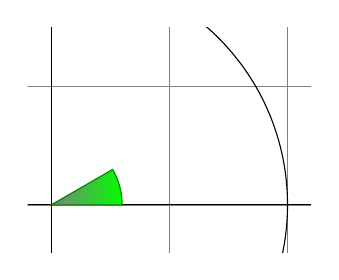
\begin{tikzpicture}[scale=3]
  \clip (-0.1,-0.2) rectangle (1.1,0.75);
  \draw[step=.5cm,gray,very thin] (-1.4,-1.4) grid (1.4,1.4);
  \draw (-1.5,0) -- (1.5,0);
  \draw (0,-1.5) -- (0,1.5);
  \draw (0,0) circle [radius=1cm];
  \shadedraw[left color=gray,right color=green, draw=green!50!black]
    (0,0) -- (3mm,0mm)
    arc [start angle=0, end angle=30, radius=3mm] -- cycle;
\end{tikzpicture}

\end{dispExample*}
\switchcolumn
\begin{dispExample*}{sidebyside}
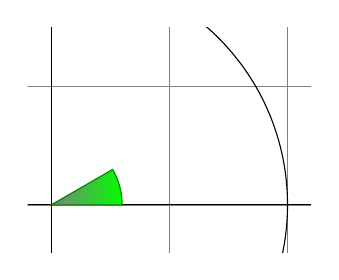
\begin{tikzpicture}[scale=3]
  \clip (-0.1,-0.2) rectangle (1.1,0.75);
  \draw[step=.5cm,gray,very thin] (-1.4,-1.4) grid (1.4,1.4);
  \draw (-1.5,0) -- (1.5,0);
  \draw (0,-1.5) -- (0,1.5);
  \draw (0,0) circle [radius=1cm];
  \shadedraw[left color=gray,right color=green, draw=green!50!black]
    (0,0) -- (3mm,0mm)
    arc [start angle=0, end angle=30, radius=3mm] -- cycle;
\end{tikzpicture}

\end{dispExample*}

\switchcolumn[0]*
However, he wisely decides that shadings usually only distract without adding
anything to the picture.
\switchcolumn
然而,他明智地决定,渐变通常只会分散注意力,而不会为图形增添任何东西。

\switchcolumn[0]*
\subsection{Specifying Coordinates}
\switchcolumn
\subsection{指定坐标}
\switchcolumn[0]*
Karl now wants to add the sine and cosine lines. He knows already that he can
use the |color=| option to set the lines' colors. So, what is the best way to
specify the coordinates?
\switchcolumn
现在Karl想要添加正弦和余弦线。他已经知道可以使用|color=|选项来设置线条的颜色。那么,最好的方法是如何指定坐标呢?
\switchcolumn[0]*
There are different ways of specifying coordinates. The easiest way is to say
something like |(10pt,2cm)|. This means 10pt in $x$-direction and 2cm in
$y$-directions. Alternatively, you can also leave out the units as in |(1,2)|,
which means ``one times the current $x$-vector plus twice the current
$y$-vector''. These vectors default to 1cm in the $x$-direction and 1cm in the
$y$-direction, respectively.
\switchcolumn
有不同的指定坐标的方法。最简单的方法是使用类似于|(10pt,2cm)|的表示方式。这表示在$x$方向上为10pt,在$y$方向上为2cm。另外,你也可以省略单位,例如|(1,2)|,它表示``当前$x$向量的一倍加上当前$y$向量的两倍''。这些向量默认分别为1cm和1cm。
\switchcolumn[0]*
In order to specify points in polar coordinates, use the notation |(30:1cm)|,
which means 1cm in direction 30 degree. This is obviously quite useful to ``get
to the point $(\cos 30^\circ,\sin 30^\circ)$ on the circle''.
\switchcolumn
为了指定极坐标中的点,可以使用|(30:1cm)|的表示方式,它表示方向为30度的1cm。这显然非常有用,可以``到达圆上的点$(\cos 30^\circ,\sin 30^\circ)$''。
\end{paracol}
极坐标是表示平面上的点的一种坐标系统。极坐标将平面上的每个点表示成 $(r,\theta)$ 的形式,其中:
\begin{itemize}
    \item $r$ 是该点到坐标原点的距离,叫做极径。
    \item $\theta$ 是该点在平面上的角度,叫做极角。极角 $\theta$ 的取值范围通常是 $[0, 2\pi)$,也可以是 $[0, 360^\circ)$。$\theta=0$ 对应正右方。
\end{itemize}


极坐标与笛卡尔坐标的转换关系为:
$ x = r\cos\theta, \quad y = r\sin\theta $

极坐标的性质和应用包括:
\begin{itemize}
    \item 极坐标通过距离原点和角度唯一确定一个点。
    \item 极坐标对于表示圆、螺线等曲线方便。
    \item 极坐标可用于表示向心力和离心力问题。
    \item 极坐标可简化表达微分方程的解析解。
    \item 极坐标在计算机图形学中也有应用。
    \item 极坐标结合复数的指数形式,可以表示复平面上的点。
\end{itemize}

总之,极坐标是除了笛卡尔坐标以外描述平面点的重要方法。它在某些问题中表达更简洁和直观。但笛卡尔坐标对于表示直线方程更方便。两者都有各自的优点。
\columnratio{0.55}
\begin{paracol}{2}
You can add a single |+| sign in front of a coordinate or two of them as in
|+(0cm,1cm)| or |++(2cm,0cm)|. Such coordinates are interpreted differently:
The first form means ``1cm upwards from the previous specified position'' and
the second means ``2cm to the right of the previous specified position, making
this the new specified position''. For example, we can draw the sine line as
follows:
\switchcolumn
你可以在坐标前面加一个单独的|+|符号,或者两个|+|符号,例如|+(0cm,1cm)|或|++(2cm,0cm)|。这些坐标的解释方式不同:第一种形式表示相对于之前指定的位置向上移动1cm'',而第二种表示相对于之前指定的位置向右移动2cm,并将其作为新指定的位置''。例如,我们可以如下绘制正弦线:
\switchcolumn[0]*
\begin{dispExample*}{sidebyside}
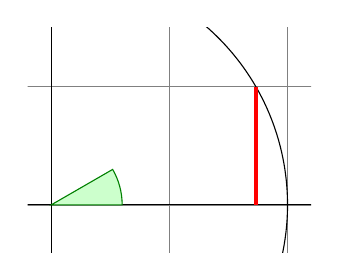
\begin{tikzpicture}[scale=3]
  \clip (-0.1,-0.2) rectangle (1.1,0.75);
  \draw[step=.5cm,gray,very thin] (-1.4,-1.4) grid (1.4,1.4);
  \draw (-1.5,0) -- (1.5,0);
  \draw (0,-1.5) -- (0,1.5);
  \draw (0,0) circle [radius=1cm];
  \filldraw[fill=green!20,draw=green!50!black] (0,0) -- (3mm,0mm)
      arc [start angle=0, end angle=30, radius=3mm] -- cycle;
  \draw[red,very thick] (30:1cm) -- +(0,-0.5);%red 表示线条的颜色为红色。very thick 表示线条的宽度为“非常粗”。(30:1cm) 指定了路径的起始点。这里使用了极坐标表示方法,其中 30 是极角,表示从水平右方向逆时针旋转30度的方向,1cm 是极径,表示从原点(通常是当前图形的(0,0)坐标)到该点的距离是1厘米。+(0,-0.5) 表示相对于前一个点的坐标。加号 + 表示这是一个相对坐标,而不是绝对坐标。这里的 (0,-0.5) 意味着从当前点向下移动0.5厘米,以创建线条的终点。
\end{tikzpicture}

\end{dispExample*}
\switchcolumn
\begin{dispExample*}{sidebyside}
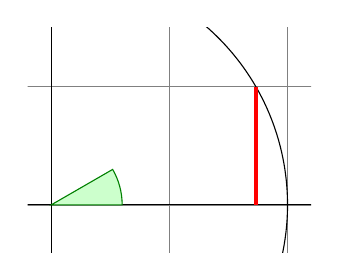
\begin{tikzpicture}[scale=3]
  \clip (-0.1,-0.2) rectangle (1.1,0.75);
  \draw[step=.5cm,gray,very thin] (-1.4,-1.4) grid (1.4,1.4);
  \draw (-1.5,0) -- (1.5,0);
  \draw (0,-1.5) -- (0,1.5);
  \draw (0,0) circle [radius=1cm];
  \filldraw[fill=green!20,draw=green!50!black] (0,0) -- (3mm,0mm)
      arc [start angle=0, end angle=30, radius=3mm] -- cycle;
  \draw[red,very thick] (30:1cm) -- +(0,-0.5);%red 表示线条的颜色为红色。very thick 表示线条的宽度为“非常粗”。(30:1cm) 指定了路径的起始点。这里使用了极坐标表示方法,其中 30 是极角,表示从水平右方向逆时针旋转30度的方向,1cm 是极径,表示从原点(通常是当前图形的(0,0)坐标)到该点的距离是1厘米。+(0,-0.5) 表示相对于前一个点的坐标。加号 + 表示这是一个相对坐标,而不是绝对坐标。这里的 (0,-0.5) 意味着从当前点向下移动0.5厘米,以创建线条的终点。
\end{tikzpicture}

\end{dispExample*}

\switchcolumn[0]*
Karl used the fact $\sin 30^\circ = 1/2$. However, he very much doubts that his
students know this, so it would be nice to have a way of specifying ``the point
straight down from |(30:1cm)| that lies on the $x$-axis''. This is, indeed,
possible using a special syntax: Karl can write \verb!(30:1cm |- 0,0)!. In
general, the meaning of |(|\meta{p}\verb! |- !\meta{q}|)| is ``the intersection
of a vertical line through $p$ and a horizontal line through $q$''.
\switchcolumn
Karl事实上使用了$\sin 30^\circ = 1/2$。然而,他非常怀疑他的学生们是否知道这一点,所以最好有一种方法来指定从|(30:1cm)|指向$x$轴下方的点''。事实上,使用一种特殊的语法是可以实现的:Karl可以写成\verb!(30:1cm |- 0,0)!。一般来说,|(|\meta{p}\verb! |- !\meta{q}|)|的意思是通过$p$的垂直线与$q$的水平线的交点''。
\switchcolumn[0]*
Next, let us draw the cosine line. One way would be to say
\verb!(30:1cm |- 0,0) -- (0,0)!. Another way is the following: we ``continue''
from where the sine ends:
\switchcolumn
接下来,让我们绘制余弦线。一种方法是说 \verb!(30:1cm |- 0,0) -- (0,0)!。另一种方法如下:我们从正弦结束的地方“继续”:
%
\switchcolumn[0]*
\begin{dispExample*}{sidebyside}
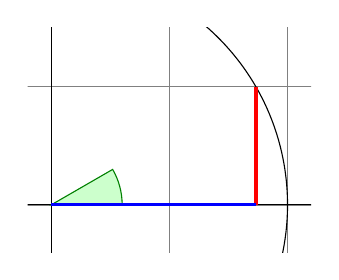
\begin{tikzpicture}[scale=3]
  \clip (-0.1,-0.2) rectangle (1.1,0.75);
  \draw[step=.5cm,gray,very thin] (-1.4,-1.4) grid (1.4,1.4);
  \draw (-1.5,0) -- (1.5,0);
  \draw (0,-1.5) -- (0,1.5);
  \draw (0,0) circle [radius=1cm];
  \filldraw[fill=green!20,draw=green!50!black] (0,0) -- (3mm,0mm)
      arc [start angle=0, end angle=30, radius=3mm] -- cycle;
  \draw[red,very thick]  (30:1cm) -- +(0,-0.5);
  \draw[blue,very thick] (30:1cm) ++(0,-0.5) -- (0,0);%(30:1cm) 使用极坐标指定了一个点的位置。这里 30 度是极角,表示从正x轴(水平向右)开始,逆时针旋转 30 度的方向;1cm 是极径,表示点距离原点的直线距离是 1 厘米。 ++(0,-0.5) 指定了一个相对于前一个点 (30:1cm) 的新位置。双加号 ++ 更改当前点的位置,这意味着新的当前点将是原来的点加上提供的坐标差。在这个例子中,它表示从 (30:1cm) 沿着 y 轴向下移动 0.5 厘米。
\end{tikzpicture}

\end{dispExample*}
\switchcolumn
\begin{dispExample*}{sidebyside}
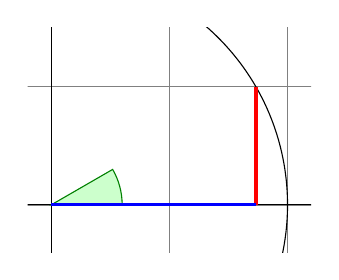
\begin{tikzpicture}[scale=3]
  \clip (-0.1,-0.2) rectangle (1.1,0.75);
  \draw[step=.5cm,gray,very thin] (-1.4,-1.4) grid (1.4,1.4);
  \draw (-1.5,0) -- (1.5,0);
  \draw (0,-1.5) -- (0,1.5);
  \draw (0,0) circle [radius=1cm];
  \filldraw[fill=green!20,draw=green!50!black] (0,0) -- (3mm,0mm)
      arc [start angle=0, end angle=30, radius=3mm] -- cycle;
  \draw[red,very thick]  (30:1cm) -- +(0,-0.5);
  \draw[blue,very thick] (30:1cm) ++(0,-0.5) -- (0,0);%(30:1cm) 使用极坐标指定了一个点的位置。这里 30 度是极角,表示从正x轴(水平向右)开始,逆时针旋转 30 度的方向;1cm 是极径,表示点距离原点的直线距离是 1 厘米。 ++(0,-0.5) 指定了一个相对于前一个点 (30:1cm) 的新位置。双加号 ++ 更改当前点的位置,这意味着新的当前点将是原来的点加上提供的坐标差。在这个例子中,它表示从 (30:1cm) 沿着 y 轴向下移动 0.5 厘米。
\end{tikzpicture}

\end{dispExample*}


\switchcolumn[0]*
Note that there is no |--| between |(30:1cm)| and |++(0,-0.5)|. In detail, this
path is interpreted as follows: ``First, the |(30:1cm)| tells me to move my pen
to $(\cos 30^\circ,1/2)$. Next, there comes another coordinate specification,
so I move my pen there without drawing anything. This new point is half a unit
down from the last position, thus it is at $(\cos 30^\circ,0)$. Finally, I move
the pen to the origin, but this time drawing something (because of the |--|).''
\switchcolumn
请注意,在 |(30:1cm)| 和 |++(0,-0.5)| 之间没有 |--|。具体来说,该路径的解释如下:``首先,|(30:1cm)| 告诉我将笔移动到 $(\cos 30^\circ,1/2)$。接下来,出现了另一个坐标指定,所以我将笔移动到那个位置,但不画任何东西。这个新点相对于上一个位置向下移动了半个单位,因此它位于 $(\cos 30^\circ,0)$。最后,我将笔移动到原点,但这次画了一些东西(因为有 |--|)''。
\switchcolumn[0]*
To appreciate the difference between |+| and |++| consider the following
example:
\switchcolumn
要理解 |+| 和 |++| 之间的区别,请考虑以下情况:
\switchcolumn[0]*
\begin{dispExample*}{sidebyside}

\begin{tikzpicture}
  \def\rectanglepath{-- ++(1cm,0cm)  -- ++(0cm,1cm)  -- ++(-1cm,0cm) -- cycle}
  \draw (0,0) \rectanglepath;
  \draw (1.5,0) \rectanglepath;
\end{tikzpicture}

\end{dispExample*}
\switchcolumn
\begin{dispExample*}{sidebyside}
\begin{tikzpicture}
  \def\rectanglepath{-- ++(1cm,0cm)  -- ++(0cm,1cm)  -- ++(-1cm,0cm) -- cycle}
  \draw (0,0) \rectanglepath;
  \draw (1.5,0) \rectanglepath;
\end{tikzpicture}

\end{dispExample*}


\switchcolumn[0]*
By comparison, when using a single |+|, the coordinates are different:
\switchcolumn
相比之下,当使用单个 |+| 时,坐标是不同的:
\switchcolumn[0]*
\begin{dispExample*}{sidebyside}
\begin{tikzpicture}
  \def\rectanglepath{-- +(1cm,0cm)  -- +(1cm,1cm)  -- +(0cm,1cm) -- cycle}
  \draw (0,0) \rectanglepath;
  \draw (1.5,0) \rectanglepath;
\end{tikzpicture}

\end{dispExample*}
\switchcolumn
\begin{dispExample*}{sidebyside}
\begin{tikzpicture}
  \def\rectanglepath{-- +(1cm,0cm)  -- +(1cm,1cm)  -- +(0cm,1cm) -- cycle}
  \draw (0,0) \rectanglepath;
  \draw (1.5,0) \rectanglepath;
\end{tikzpicture}

\end{dispExample*}


\switchcolumn[0]*
Naturally, all of this could have been written more clearly and more
economically like this (either with a single or a double |+|):
\switchcolumn
当然,所有这些都可以更清晰、更简洁地写成这样(无论是使用单个还是双个 |+|):
\switchcolumn[0]*
\begin{dispExample*}{sidebyside}
\tikz \draw (0,0) rectangle +(1,1)  (1.5,0) rectangle +(1,1);

\end{dispExample*}
\switchcolumn
\begin{dispExample*}{sidebyside}
\tikz \draw (0,0) rectangle +(1,1)  (1.5,0) rectangle +(1,1);

\end{dispExample*}


\switchcolumn[0]*
\subsection{Intersecting Paths}
\switchcolumn
\subsection{相交路径}
\switchcolumn[0]*
Karl is left with the line for $\tan \alpha$, which seems difficult to specify
using transformations and polar coordinates. The first -- and easiest -- thing
he can do is so simply use the coordinate |(1,{tan(30)})| since \tikzname's
math engine knows how to compute things like |tan(30)|. Note the added braces
since, otherwise, \tikzname's parser would think that the first closing
parenthesis ends the coordinate (in general, you need to add braces around
components of coordinates when these components contain parentheses).
\switchcolumn
Karl要一个表示$\tan \alpha$的直线,用变换和极坐标似乎比较困难。他可以简单地使用坐标 |(1,{tan(30)})|,因为\tikzname 的数学引擎知道如何计算类似|tan(30)|的表达式。请注意,要加上花括号,否则\tikzname 的解析器会认为第一个闭括号结束了坐标(通常情况下,当坐标的组成部分包含括号时,需要在其周围加上花括号)。
\switchcolumn[0]*
Karl can, however, also use a more elaborate, but also more ``geometric'' way
of computing the length of the orange line: He can specify intersections of
paths as coordinates. The line for $\tan \alpha$ starts at $(1,0)$ and goes
upward to a point that is at the intersection of a line going ``up'' and a line
going from the origin through |(30:1cm)|. Such computations are made available
by the |intersections| library.
\switchcolumn
然而,Karl也可以使用一种更复杂、更“几何”的方式来计算橙色线段的长度:他可以将路径的交点指定为坐标。表示$\tan \alpha$的线段从$(1,0)$开始向上延伸,直到一个点,该点是向“上”延伸的线和经过原点的经过|(30:1cm)|的线的交点。这样的计算可以通过|intersections|库来实现。
\switchcolumn[0]*
What Karl must do is to create two ``invisible'' paths that intersect at the
position of interest. Creating paths that are not otherwise seen can be done
using the |\path| command without any options like |draw| or |fill|. Then, Karl
can add the |name path| option to the path for later reference. Once the paths
have been constructed, Karl can use the |name intersections| to assign names to
the coordinate for later reference.
\switchcolumn
Karl需要做的是创建两条在感兴趣位置相交的“不可见”路径。使用不带任何选项(如|draw|或|fill|)的|\path|命令可以创建不可见的路径。然后,Karl可以为路径添加|name path|选项以供以后引用。一旦构建完路径,Karl可以使用|name intersections|为坐标赋予名称以供以后引用。
\switchcolumn[0]*
\begin{codeexample}[code only]
\path [name path=upward line] (1,0) -- (1,1);
\path [name path=sloped line] (0,0) -- (30:1.5cm); % a bit longer, so that there is an intersection

% (add `\usetikzlibrary{intersections}' after loading tikz in the preamble)
\draw [name intersections={of=upward line and sloped line, by=x}]
  [very thick,orange] (1,0) -- (x);
\end{codeexample}

\switchcolumn[0]*
\subsection{Adding Arrow Tips}
\switchcolumn
\subsection{添加箭头标记}
\switchcolumn[0]*
Karl now wants to add the little arrow tips at the end of the axes. He has
noticed that in many plots, even in scientific journals, these arrow tips seem
to be missing, presumably because the generating programs cannot produce them.
Karl thinks arrow tips belong at the end of axes. His son agrees. His students
do not care about arrow tips.
\switchcolumn
Karl现在想在坐标轴的末端添加一些小箭头标记。他注意到在许多绘图中,即使在科学期刊中,这些箭头标记似乎也缺失了,可能是因为生成程序无法产生它们。Karl认为箭头标记应该放在坐标轴的末端。他的儿子也同意。他的学生们则对箭头标记不感兴趣。
\switchcolumn[0]*
It turns out that adding arrow tips is pretty easy: Karl adds the option |->|
to the drawing commands for the axes:
\switchcolumn
添加箭头标记其实非常简单:Karl只需在绘制坐标轴的命令中添加选项|->|:
\switchcolumn[0]*
\begin{codeexample}[preamble={\usetikzlibrary{intersections}}]
\begin{tikzpicture}[scale=3]
  \clip (-0.1,-0.2) rectangle (1.1,1.51);
  \draw[step=.5cm,gray,very thin] (-1.4,-1.4) grid (1.4,1.4);
  \draw[->] (-1.5,0) -- (1.5,0);
  \draw[->] (0,-1.5) -- (0,1.5);
  \draw (0,0) circle [radius=1cm];
  \filldraw[fill=green!20,draw=green!50!black] (0,0) -- (3mm,0mm)
        arc [start angle=0, end angle=30, radius=3mm] -- cycle;
  \draw[red,very thick]    (30:1cm) -- +(0,-0.5);
  \draw[blue,very thick]   (30:1cm) ++(0,-0.5) -- (0,0);

  \path [name path=upward line] (1,0) -- (1,1);
  \path [name path=sloped line] (0,0) -- (30:1.5cm);
  \draw [name intersections={of=upward line and sloped line, by=x}]
        [very thick,orange] (1,0) -- (x);
\end{tikzpicture}
\end{codeexample}
\switchcolumn[0]*
If Karl had used the option |<-| instead of |->|, arrow tips would have been
put at the beginning of the path. The option |<->| puts arrow tips at both ends
of the path.
\switchcolumn
如果卡尔使用选项 |<-| 而不是 |->|,箭头将会放在路径的起始位置。选项 |<->| 在路径的两端放置箭头。
\switchcolumn[0]*
There are certain restrictions to the kind of paths to which arrow tips can be
added. As a rule of thumb, you can add arrow tips only to a single open
``line''. For example, you cannot add tips to, say, a rectangle or a circle.
However, you can add arrow tips to curved paths and to paths that have several
segments, as in the following examples:
\switchcolumn
对于可以添加箭头的路径类型有一些限制。一般来说,你只能在一个单独的“线段”上添加箭头。例如,你不能在矩形或圆形上添加箭头。但是,你可以在曲线路径和具有多个线段的路径上添加箭头,如下面的示例所示:
\switchcolumn[0]*
\begin{dispExample*}{sidebyside}
\begin{tikzpicture}
  \draw [<->] (0,0) arc [start angle=180, end angle=30, radius=10pt];
  \draw [<->] (1,0) -- (1.5cm,10pt) -- (2cm,0pt) -- (2.5cm,10pt);
\end{tikzpicture}

\end{dispExample*}
\switchcolumn
\begin{dispExample*}{sidebyside}
\begin{tikzpicture}
  \draw [<->] (0,0) arc [start angle=180, end angle=30, radius=10pt];
  \draw [<->] (1,0) -- (1.5cm,10pt) -- (2cm,0pt) -- (2.5cm,10pt);
\end{tikzpicture}

\end{dispExample*}

\switchcolumn[0]*
Karl has a more detailed look at the arrow that \tikzname\ puts at the end. It
looks like this when he zooms it: \tikz[baseline] \draw[->,line width=1pt]
(0pt,.5ex) -- ++(10pt,0pt);. The shape seems vaguely familiar and, indeed, this
is exactly the end of \TeX's standard arrow used in something like $f\colon A
\to B$.
\switchcolumn
卡尔仔细观察了 \tikzname\ 放在路径末端的箭头。当他放大观察时,它看起来是这样的:\tikz[baseline] \draw[->,line width=1pt] (0pt,.5ex) -- ++(10pt,0pt);。这个形状似乎有点熟悉,实际上,这正是类似于 $f\colon A \to B$ 中 \TeX\ 标准箭头的末端。
\switchcolumn[0]*
Karl likes the arrow, especially since it is not ``as thick'' as the arrows
offered by many other packages. However, he expects that, sometimes, he might
need to use some other kinds of arrow. To do so, Karl can say |>=|\meta{kind of
end arrow tip}, where \meta{kind of end arrow tip} is a special arrow tip
specification. For example, if Karl says |>=Stealth|, then he tells \tikzname\
that he would like  ``stealth-fighter-like'' arrow tips:
\todosp{remaining instance of bug \#473}
\switchcolumn
卡尔喜欢这个箭头,特别是它不像其他许多包提供的箭头那么“粗”。然而,他预计有时可能需要使用其他类型的箭头。为了这样做,卡尔可以使用 |>=|\meta{箭头类型},其中 \meta{箭头类型} 是一种特殊的箭头类型说明。例如,如果卡尔使用 |>=Stealth|,则表示他想要“隐形战斗机”样式的箭头:
\switchcolumn[0]*
\begin{codeexample}[preamble={\usetikzlibrary{arrows.meta}}]
\begin{tikzpicture}[>=Stealth]
  \draw [->] (0,0) arc [start angle=180, end angle=30, radius=10pt];
  \draw [<<-,very thick] (1,0) -- (1.5cm,10pt) -- (2cm,0pt) -- (2.5cm,10pt);
\end{tikzpicture}
\end{codeexample}
\switchcolumn[0]*
Karl wonders whether such a military name for the arrow type is really
necessary. He is not really mollified when his son tells him that Microsoft's
PowerPoint uses the same name. He decides to have his students discuss this at
some point.
\switchcolumn
卡尔想知道是否真的有必要给箭头类型取一个军事名称。当他的儿子告诉他微软的 PowerPoint 也使用相同的名称时,他并没有完全安心。他决定在某个时候让学生们讨论这个问题。
\switchcolumn[0]*
In addition to |Stealth| there are several other predefined kinds of arrow tips
Karl can choose from, see Section~\ref{section-arrows}. Furthermore, he can
define arrows types himself, if he needs new ones.
\switchcolumn
除了 |Stealth|,卡尔还可以从几种预定义的箭头类型中进行选择,详见第~\ref{section-arrows}节。此外,如果需要,他还可以自定义箭头类型。

\switchcolumn[0]*
\subsection{Scoping}
\switchcolumn
\subsection{作用范围}
\switchcolumn[0]*
Karl saw already that there are numerous graphic options that affect how paths
are rendered. Often, he would like to apply certain options to a whole set of
graphic commands. For example, Karl might wish to draw three paths using a
|thick| pen, but would like everything else to be drawn ``normally''.
\switchcolumn
卡尔已经注意到有许多图形选项会影响路径的渲染方式。通常情况下,他希望将某些选项应用到一整组图形命令中。例如,卡尔可能希望使用粗线绘制三条路径,但希望其他所有东西都以“正常”的方式绘制。
\switchcolumn[0]*
If Karl wishes to set a certain graphic option for the whole picture, he can
simply pass this option to the |\tikz| command or to the |{tikzpicture}|
environment (Gerda would pass the options to |\tikzpicture| and Hans passes
them to |\starttikzpicture|). However, if Karl wants to apply graphic options
to a local group, he put these commands inside a |{scope}| environment (Gerda
uses |\scope| and |\endscope|, Hans uses |\startscope| and |\stopscope|). This
environment takes graphic options as an optional argument and these options
apply to everything inside the scope, but not to anything outside.
\switchcolumn
如果卡尔希望为整个图形设置某个图形选项,他可以将该选项直接传递给 |\tikz| 命令或 |{tikzpicture}| 环境(格尔达会将选项传递给 |\tikzpicture|,汉斯会将选项传递给 |\starttikzpicture|)。然而,如果卡尔想要将图形选项应用于局部分组,他可以将这些命令放在 |{scope}| 环境内(格尔达使用 |\scope| 和 |\endscope|,汉斯使用 |\startscope| 和 |\stopscope|)。这个环境接受一个可选的图形选项参数,并且这些选项应用于范围内的所有内容,但不影响范围外的内容。
\switchcolumn[0]*
Here is an example:
\switchcolumn
以下是一个示例:
\switchcolumn[0]*
\begin{dispExample*}{sidebyside}
\begin{tikzpicture}[ultra thick]
  \draw (0,0) -- (0,1);
  \begin{scope}[thin]
    \draw (1,0) -- (1,1);
    \draw (2,0) -- (2,1);
  \end{scope}
  \draw (3,0) -- (3,1);
\end{tikzpicture}

\end{dispExample*}
\switchcolumn
\begin{dispExample*}{sidebyside}
\begin{tikzpicture}[ultra thick]
  \draw (0,0) -- (0,1);
  \begin{scope}[thin]
    \draw (1,0) -- (1,1);
    \draw (2,0) -- (2,1);
  \end{scope}
  \draw (3,0) -- (3,1);
\end{tikzpicture}

\end{dispExample*}

\switchcolumn[0]*
Scoping has another interesting effect: Any changes to the clipping area are
local to the scope. Thus, if you say |\clip| somewhere inside a scope, the
effect of the |\clip| command ends at the end of the scope. This is useful
since there is no other way of ``enlarging'' the clipping area.
\switchcolumn
作用范围还有另一个有趣的效果:对裁剪区域的任何更改都仅限于该范围内。因此,如果你在某个作用范围内使用 |\clip| 命令,它的效果将在作用范围结束时结束。这是有用的,因为没有其他方法“扩大”裁剪区域。
\switchcolumn[0]*
Karl has also already seen that giving options to commands like |\draw| apply
only to that command. It turns out that the situation is slightly more complex.
First, options to a command like |\draw| are not really options to the command,
but they are ``path options'' and can be given anywhere on the path. So,
instead of |\draw[thin] (0,0) -- (1,0);| one can also write
|\draw (0,0) [thin] -- (1,0);| or |\draw (0,0) -- (1,0) [thin];|; all of these
have the same effect. This might seem strange since in the last case, it would
appear that the |thin| should take effect only ``after'' the line from $(0,0)$
to $(1,0)$ has been drawn. However, most graphic options only apply to the
whole path. Indeed, if you say both |thin| and |thick| on the same path, the
last option given will ``win''.
\switchcolumn
卡尔已经注意到,给类似 |\draw| 的命令添加选项只对该命令起作用。事实证明,情况稍微复杂一些。首先,给 |\draw| 这样的命令添加的选项实际上不是该命令的选项,而是“路径选项”,可以在路径的任何位置给出。因此,可以用 |\draw[thin] (0,0) -- (1,0);|,也可以写作 |\draw (0,0) [thin] -- (1,0);| 或 |\draw (0,0) -- (1,0) [thin];|;所有这些都具有相同的效果。这可能看起来有些奇怪,因为在最后一种情况下,似乎 |thin| 应该只在从 $(0,0)$ 到 $(1,0)$ 的线段绘制“之后”才生效。然而,大多数图形选项只适用于整个路径。实际上,如果在同一路径上同时使用 |thin| 和 |thick|,最后给出的选项将“胜出”。
\switchcolumn[0]*
When reading the above, Karl notices that only ``most'' graphic options apply
to the whole path. Indeed, all transformation options do \emph{not} apply to
the whole path, but only to ``everything following them on the path''. We will
have a more detailed look at this in a moment. Nevertheless, all options given
during a path construction apply only to this path.
\switchcolumn
在阅读上述内容时,卡尔注意到只有“大多数”图形选项适用于整个路径。实际上,所有的变换选项\emph{不}适用于整个路径,而是只适用于“路径上紧随其后的所有内容”。我们稍后将详细研究这个问题。然而,路径构造过程中给出的所有选项都只适用于该路径。

\switchcolumn[0]*
\subsection{Transformations}
\switchcolumn
\subsection{变换}
\switchcolumn[0]*
When you specify a  coordinate like |(1cm,1cm)|, where is that coordinate
placed on the page? To determine the position, \tikzname, \TeX, and
\textsc{pdf} or PostScript all apply certain transformations to the given
coordinate in order to determine the final position on the page.
\switchcolumn
当你指定一个像 |(1cm,1cm)| 这样的坐标时,该坐标在页面上的哪个位置?为了确定位置,\tikzname、\TeX 和 \textsc{pdf} 或 PostScript 都会对给定的坐标应用一定的变换,以确定最终在页面上的位置。
\switchcolumn[0]*
\tikzname\ provides numerous options that allow you to transform coordinates in
\tikzname's private coordinate system. For example, the |xshift| option allows
you to shift all subsequent points by a certain amount:
\switchcolumn
\tikzname\ 提供了许多选项,允许你在\tikzname 的私有坐标系统中进行坐标变换。例如,|xshift| 选项允许你将所有后续点向右平移一定量:
\switchcolumn[0]*
\begin{dispExample*}{sidebyside}
\tikz \draw (0,0) -- (0,0.5) [xshift=2pt] (0,0) -- (0,0.5);

\end{dispExample*}
\switchcolumn
\begin{dispExample*}{sidebyside}
\tikz \draw (0,0) -- (0,0.5) [xshift=2pt] (0,0) -- (0,0.5);

\end{dispExample*}

\switchcolumn[0]*
It is important to note that you can change transformation ``in the middle of a
path'', a feature that is not supported by \pdf\ or PostScript. The reason is
that \tikzname\ keeps track of its own transformation matrix.
\switchcolumn
重要的是要注意,你可以在“路径中间”更改变换,而这是\pdf\ 或 PostScript 不支持的功能。原因是\tikzname\ 跟踪自己的变换矩阵。
\switchcolumn[0]*
Here is a more complicated example:
\switchcolumn
以下是一个更复杂的例子:
\switchcolumn[0]*
\begin{dispExample*}{sidebyside}
\begin{tikzpicture}[even odd rule,rounded corners=2pt,x=10pt,y=10pt]
  \filldraw[fill=yellow!80!black] (0,0)   rectangle (1,1)
        [xshift=5pt,yshift=5pt]   (0,0)   rectangle (1,1)
                    [rotate=30]   (-1,-1) rectangle (2,2);
\end{tikzpicture}

\end{dispExample*}
\switchcolumn
\begin{dispExample*}{sidebyside}
\begin{tikzpicture}[even odd rule,rounded corners=2pt,x=10pt,y=10pt]
  \filldraw[fill=yellow!80!black] (0,0)   rectangle (1,1)
        [xshift=5pt,yshift=5pt]   (0,0)   rectangle (1,1)
                    [rotate=30]   (-1,-1) rectangle (2,2);
\end{tikzpicture}

\end{dispExample*}

\switchcolumn[0]*
The most useful transformations are |xshift| and |yshift| for shifting, |shift|
for shifting to a given point as in |shift={(1,0)}| or |shift={+(0,0)}| (the
braces are necessary so that \TeX\ does not mistake the comma for separating
options), |rotate| for rotating by a certain angle (there is also a
|rotate around| for rotating around a given point), |scale| for scaling by a
certain factor, |xscale| and |yscale| for scaling only in the $x$- or
$y$-direction (|xscale=-1| is a flip), and |xslant| and |yslant| for slanting.
If these transformation and those that I have not mentioned are not sufficient,
the |cm| option allows you to apply an arbitrary transformation matrix. Karl's
students, by the way, do not know what a transformation matrix is.
\switchcolumn
最常用的变换 |xshift| 和 |yshift| 用于平移,|shift| 用于平移到给定点,如 |shift={(1,0)}| 或 |shift={+(0,0)}|(大括号是必需的,以免\TeX\ 将逗号误认为是选项分隔符),|rotate| 用于按一定角度旋转(还有一个 |rotate around| 用于围绕给定点旋转),|scale| 用于按一定比例缩放,|xscale| 和 |yscale| 用于仅在$x$-方向或$y$-方向缩放(|xscale=-1| 是翻转),|xslant| 和 |yslant| 用于倾斜。如果这些变换和我没有提到的其他变换不足够使用,|cm| 选项允许你应用任意的变换矩阵。顺便说一下,卡尔的学生们并不知道什么是变换矩阵。

\switchcolumn[0]*
\subsection{Repeating Things: For-Loops}
\switchcolumn
\subsection{重复操作:For循环}
\switchcolumn[0]*
Karl's next aim is to add little ticks on the axes at positions $-1$, $-1/2$,
$1/2$, and $1$. For this, it would be nice to use some kind of ``loop'',
especially since he wishes to do the same thing at each of these positions.
There are different packages for doing this. \LaTeX\ has its own internal
command for this, |pstricks| comes along with the powerful |\multido| command.
All of these can be used together with \tikzname, so if you are familiar with
them, feel free to use them. \tikzname\ introduces yet another command, called
|\foreach|, which I introduced since I could never remember the syntax of the
other packages. |\foreach| is defined in the package |pgffor| and can be used
independently of \tikzname, but \tikzname\ includes it automatically.
\switchcolumn
Karl的下一个目标是在坐标轴上添加小刻度,位置分别为$-1$,$-1/2$,$1/2$和$1$。为此,最好使用一种``循环''机制,特别是因为他希望在每个位置上执行相同的操作。有不同的包可以实现这一点。\LaTeX 内部有自己的命令,|pstricks| 包则提供了强大的 |\multido| 命令。所有这些命令都可以与 \tikzname\ 一起使用,所以如果你熟悉它们,可以随意使用。\tikzname\ 还引入了另一个命令,称为 |\foreach|,我引入它是因为我总是记不住其他包的语法。|\foreach| 定义在 |pgffor| 包中,可以独立于 \tikzname\ 使用,但 \tikzname\ 会自动包含它。
\switchcolumn[0]*
In its basic form, the |\foreach| command is easy to use:
\switchcolumn
|\foreach| 命令的基本用法很简单:
\switchcolumn[0]*
\begin{dispExample*}{sidebyside}
\foreach \x in {1,2,3} {$x =\x$, }

\end{dispExample*}
\switchcolumn
\begin{dispExample*}{sidebyside}
\foreach \x in {1,2,3} {$x =\x$, }

\end{dispExample*}


\switchcolumn[0]*
The general syntax is
|\foreach| \meta{variable}| in {|\meta{list of values}|} |\meta{commands}.
Inside the \meta{commands}, the \meta{variable} will be assigned to the
different values. If the \meta{commands} do not start with a brace, everything
up to the next semicolon is used as \meta{commands}.
\switchcolumn
它的一般语法是
|\foreach| \meta{变量}| in {|\meta{值列表}|} |\meta{命令}。
在 \meta{命令} 中,\meta{变量} 将被赋予不同的值。如果 \meta{命令} 不以大括号开头,那么直到下一个分号之前的所有内容都将用作 \meta{命令}。
\switchcolumn[0]*
For Karl and the ticks on the axes, he could use the following code:
\switchcolumn
对于Karl和坐标轴上的刻度,他可以使用以下代码:
\switchcolumn[0]*
\begin{dispExample*}{sidebyside}
\begin{tikzpicture}[scale=3]
  \clip (-0.1,-0.2) rectangle (1.1,1.51);
  \draw[step=.5cm,gray,very thin] (-1.4,-1.4) grid (1.4,1.4);
  \filldraw[fill=green!20,draw=green!50!black] (0,0) -- (3mm,0mm)
      arc [start angle=0, end angle=30, radius=3mm] -- cycle;
  \draw[->] (-1.5,0) -- (1.5,0);
  \draw[->] (0,-1.5) -- (0,1.5);
  \draw (0,0) circle [radius=1cm];

  \foreach \x in {-1cm,-0.5cm,1cm}
    \draw (\x,-1pt) -- (\x,1pt);
  \foreach \y in {-1cm,-0.5cm,0.5cm,1cm}
    \draw (-1pt,\y) -- (1pt,\y);
\end{tikzpicture}

\end{dispExample*}
\switchcolumn
\begin{dispExample*}{sidebyside}
\begin{tikzpicture}[scale=3]
  \clip (-0.1,-0.2) rectangle (1.1,1.51);
  \draw[step=.5cm,gray,very thin] (-1.4,-1.4) grid (1.4,1.4);
  \filldraw[fill=green!20,draw=green!50!black] (0,0) -- (3mm,0mm)
      arc [start angle=0, end angle=30, radius=3mm] -- cycle;
  \draw[->] (-1.5,0) -- (1.5,0);
  \draw[->] (0,-1.5) -- (0,1.5);
  \draw (0,0) circle [radius=1cm];

  \foreach \x in {-1cm,-0.5cm,1cm}
    \draw (\x,-1pt) -- (\x,1pt);
  \foreach \y in {-1cm,-0.5cm,0.5cm,1cm}
    \draw (-1pt,\y) -- (1pt,\y);
\end{tikzpicture}

\end{dispExample*}

\switchcolumn[0]*
As a matter of fact, there are many different ways of creating the ticks. For
example, Karl could have put the |\draw ...;| inside curly braces. He could
also have used, say,
\switchcolumn
事实上,有许多不同的方法可以创建刻度。例如,Karl可以将 |\draw ...;| 放在大括号中。他也可以使用以下方式:

\switchcolumn[0]*
\begin{codeexample}[code only]
\foreach \x in {-1,-0.5,1}
  \draw[xshift=\x cm] (0pt,-1pt) -- (0pt,1pt);
\end{codeexample}
\switchcolumn[0]*
Karl is curious what would happen in a more complicated situation where there
are, say, 20 ticks. It seems bothersome to explicitly mention all these numbers
in the set for |\foreach|. Indeed, it is possible to use |...| inside the
|\foreach| statement to iterate over a large number of values (which must,
however, be dimensionless real numbers) as in the following example:
\switchcolumn
Karl很好奇在更复杂的情况下会发生什么,比如有20个刻度。在 |\foreach| 中显式提及所有这些数字似乎很麻烦。的确,可以在 |\foreach| 语句中使用 |...| 来迭代一大堆值(但这些值必须是无量纲实数),如下面的例子所示:
\switchcolumn[0]*
\begin{dispExample*}{sidebyside}
\tikz \foreach \x in {1,...,10}
        \draw (\x,0) circle (0.4cm);

\end{dispExample*}
\switchcolumn
\begin{dispExample*}{sidebyside}
\tikz \foreach \x in {1,...,10}
        \draw (\x,0) circle (0.4cm);

\end{dispExample*}

\switchcolumn[0]*
If you provide \emph{two} numbers before the |...|, the |\foreach| statement
will use their difference for the stepping:
\switchcolumn
如果在 |...| 前提供\emph{两个}数字,|\foreach| 语句将使用它们的差值作为步长:
\switchcolumn[0]*
\begin{dispExample*}{sidebyside}
\tikz \foreach \x in {-1,-0.5,...,1}
       \draw (\x cm,-1pt) -- (\x cm,1pt);

\end{dispExample*}
\switchcolumn
\begin{dispExample*}{sidebyside}
\tikz \foreach \x in {-1,-0.5,...,1}
       \draw (\x cm,-1pt) -- (\x cm,1pt);

\end{dispExample*}

\switchcolumn[0]*
We can also nest loops to create interesting effects:
\switchcolumn
我们还可以嵌套循环以创建有趣的效果:
\switchcolumn[0]*
\begin{dispExample*}{sidebyside}
\begin{tikzpicture}
  \foreach \x in {1,2,...,5,7,8,...,12}
    \foreach \y in {1,...,5}
    {
      \draw (\x,\y) +(-.5,-.5) rectangle ++(.5,.5);
      \draw (\x,\y) node{\x,\y};
    }
\end{tikzpicture}

\end{dispExample*}
\switchcolumn
\begin{dispExample*}{sidebyside}
\begin{tikzpicture}
  \foreach \x in {1,2,...,5,7,8,...,12}
    \foreach \y in {1,...,5}
    {
      \draw (\x,\y) +(-.5,-.5) rectangle ++(.5,.5);
      \draw (\x,\y) node{\x,\y};
    }
\end{tikzpicture}

\end{dispExample*}

\switchcolumn[0]*
The |\foreach| statement can do even trickier stuff, but the above gives the
idea.
\switchcolumn
|\foreach| 语句甚至可以执行更复杂的操作,但以上内容已经给出了基本思路。

\switchcolumn[0]*
\subsection{Adding Text}
\switchcolumn
\subsection{添加文本}
\switchcolumn[0]*
Karl is, by now, quite satisfied with the picture. However, the most important
parts, namely the labels, are still missing!
\switchcolumn
卡尔对图片已经相当满意了。然而,最重要的部分,也就是标签,还是缺失的!
\switchcolumn[0]*
\tikzname\ offers an easy-to-use and powerful system for adding text and, more
generally, complex shapes to a picture at specific positions. The basic idea is
the following: When \tikzname\ is constructing a path and encounters the
keyword |node| in the middle of a path, it reads a \emph{node specification}.
The keyword |node| is typically followed by some options and then some text
between curly braces. This text is put inside a normal \TeX\ box (if the node
specification directly follows a coordinate, which is usually the case,
\tikzname\ is able to perform some magic so that it is even possible to use
verbatim text inside the boxes) and then placed at the current position, that
is, at the last specified position (possibly shifted a bit, according to the
given options). However, all nodes are drawn only after the path has been
completely drawn/filled/shaded/clipped/whatever.
\switchcolumn
\tikzname\ 提供了一个易于使用且功能强大的系统,用于在特定位置向图片添加文本和其他复杂形状。基本思想如下:当 \tikzname\ 构建路径并在路径中间遇到关键字 |node| 时,它会读取一个\emph{节点规范}。关键字 |node| 通常后面跟着一些选项,然后是花括号内的一些文本。这个文本被放入一个普通的 \TeX\ 盒子中(如果节点规范直接跟在坐标后面,这通常是情况,\tikzname\ 能够执行一些魔法,使得甚至可以在盒子中使用抄录文本),然后放置在当前位置,即最后指定的位置(根据给定的选项可能会稍微偏移一点)。然而,所有的节点都是在路径完全绘制/填充/着色/裁剪/等等之后绘制的。
\switchcolumn[0]*
\begin{dispExample*}{sidebyside}
\begin{tikzpicture}
  \draw (0,0) rectangle (2,2);
  \draw (0.5,0.5) node [fill=yellow!80!black]
                       {Text at \verb!node 1!}
     -- (1.5,1.5) node {Text at \verb!node 2!};
\end{tikzpicture}

\end{dispExample*}
\switchcolumn
\begin{dispExample*}{sidebyside}
\begin{tikzpicture}
  \draw (0,0) rectangle (2,2);
  \draw (0.5,0.5) node [fill=yellow!80!black]
                       {Text at \verb!node 1!}
     -- (1.5,1.5) node {Text at \verb!node 2!};
\end{tikzpicture}

\end{dispExample*}

\switchcolumn[0]*
Obviously, Karl would not only like to place nodes \emph{on} the last specified
position, but also to the left or the right of these positions. For this, every
node object that you put in your picture is equipped with several
\emph{anchors}. For example, the |north| anchor is in the middle at the upper
end of the shape, the |south| anchor is at the bottom and the |north east|
anchor is in the upper right corner. When you give the option |anchor=north|,
the text will be placed such that this northern anchor will lie on the current
position and the text is, thus, below the current position. Karl uses this to
draw the ticks as follows:
\switchcolumn
显然,卡尔不仅希望将节点放在最后指定的位置上,还希望将其放在这些位置的左侧或右侧。为此,你在图片中放置的每个节点对象都配备了若干\emph{锚点}。例如,|north| 锚点位于形状的上端中间,|south| 锚点位于底部,|north east| 锚点位于右上角。当给定选项 |anchor=north| 时,文本将被放置在该北方锚点上,因此文本位于当前位置的下方。卡尔使用以下方法绘制刻度线:
\switchcolumn[0]*
\begin{dispExample*}{sidebyside}
\begin{tikzpicture}[scale=3]
  \clip (-0.6,-0.2) rectangle (0.6,1.51);
  \draw[step=.5cm,help lines] (-1.4,-1.4) grid (1.4,1.4);
  \filldraw[fill=green!20,draw=green!50!black] (0,0) -- (3mm,0mm)
    arc [start angle=0, end angle=30, radius=3mm] -- cycle;
  \draw[->] (-1.5,0) -- (1.5,0);   \draw[->] (0,-1.5) -- (0,1.5);
  \draw (0,0) circle [radius=1cm];

  \foreach \x in {-1,-0.5,1}
    \draw (\x cm,1pt) -- (\x cm,-1pt) node[anchor=north] {$\x$};
  \foreach \y in {-1,-0.5,0.5,1}
    \draw (1pt,\y cm) -- (-1pt,\y cm) node[anchor=east] {$\y$};
\end{tikzpicture}

\end{dispExample*}
\switchcolumn
\begin{dispExample*}{sidebyside}
\begin{tikzpicture}[scale=3]
  \clip (-0.6,-0.2) rectangle (0.6,1.51);
  \draw[step=.5cm,help lines] (-1.4,-1.4) grid (1.4,1.4);
  \filldraw[fill=green!20,draw=green!50!black] (0,0) -- (3mm,0mm)
    arc [start angle=0, end angle=30, radius=3mm] -- cycle;
  \draw[->] (-1.5,0) -- (1.5,0);   \draw[->] (0,-1.5) -- (0,1.5);
  \draw (0,0) circle [radius=1cm];

  \foreach \x in {-1,-0.5,1}
    \draw (\x cm,1pt) -- (\x cm,-1pt) node[anchor=north] {$\x$};
  \foreach \y in {-1,-0.5,0.5,1}
    \draw (1pt,\y cm) -- (-1pt,\y cm) node[anchor=east] {$\y$};
\end{tikzpicture}

\end{dispExample*}

\switchcolumn[0]*
This is quite nice, already. Using these anchors, Karl can now add most of the
other text elements. However, Karl thinks that, though ``correct'', it is quite
counter-intuitive that in order to place something \emph{below} a given point,
he has to use the \emph{north} anchor. For this reason, there is an option
called |below|, which does the same as |anchor=north|. Similarly, |above right|
does the same as |anchor=south west|. In addition, |below| takes an optional
dimension argument. If given, the shape will additionally be shifted downwards
by the given amount. So, |below=1pt| can be used to put a text label below some
point and, additionally shift it  1pt downwards.
\switchcolumn
这已经相当不错了。使用这些锚点,Karl现在可以添加大部分其他的文本元素了。然而,Karl认为,尽管“正确”,但要在给定点的下方放置某物,他必须使用“north”锚点,这是相当不直观的。因此,有一个名为|below|的选项,它与|anchor=north|的作用相同。类似地,|above right|与|anchor=south west|的作用相同。此外,|below|接受一个可选的尺寸参数。如果给定,形状将额外向下移动给定的量。因此,可以使用|below=1pt|将文本标签放置在某个点的下方,并将其额外向下移动1pt。
\switchcolumn[0]*
Karl is not quite satisfied with the ticks. He would like to have $1/2$ or
$\frac{1}{2}$ shown instead of $0.5$, partly to show off the nice capabilities
of \TeX\ and \tikzname, partly because for positions like $1/3$ or $\pi$ it is
certainly very much preferable to have the ``mathematical'' tick there instead
of just the ``numeric'' tick. His students, on the other hand, prefer $0.5$
over $1/2$ since they are not too fond of fractions in general.
\switchcolumn
Karl对刻度线还不太满意。他想要显示$1/2$或$\frac{1}{2}$,而不是$0.5$,部分是为了展示\TeX 和\tikzname 的出色功能,部分是因为对于类似$1/3$或$\pi$的位置,使用“数学”的刻度线肯定比仅仅使用“数字”的刻度线更好。然而,他的学生们更喜欢$0.5$而不是$1/2$,因为他们对分数不太感兴趣。
\switchcolumn[0]*
Karl now faces a problem: For the |\foreach| statement, the position |\x|
should still be given as |0.5| since \tikzname\ will not know where
|\frac{1}{2}| is supposed to be. On the other hand, the typeset text should
really be  |\frac{1}{2}|. To solve this problem, |\foreach| offers a special
syntax: Instead of having one variable |\x|, Karl can specify two (or even
more) variables separated by a slash as in |\x / \xtext|. Then, the elements in
the set over which |\foreach| iterates must also be of the form
\meta{first}|/|\meta{second}. In each iteration, |\x| will be set to
\meta{first} and |\xtext| will be set to \meta{second}. If no \meta{second} is
given, the \meta{first} will be used again. So, here is the new code for the
ticks:
\switchcolumn
现在Karl面临一个问题:对于|\foreach|语句,位置|\x|仍然应该给定为|0.5|,因为\tikzname 不知道|\frac{1}{2}|应该在哪里。另一方面,排版的文本应该真正是|\frac{1}{2}|。为了解决这个问题,|\foreach|提供了一种特殊的语法:Karl可以指定两个(甚至更多)由斜杠分隔的变量,如|\x / \xtext|。然后,|\foreach|迭代的集合中的元素必须以\meta{first}|/|\meta{second}的形式。在每次迭代中,|\x|将被设置为\meta{first},|\xtext|将被设置为\meta{second}。如果没有给出\meta{second},则再次使用\meta{first}。因此,这是刻度线的新代码:
\switchcolumn[0]*
\begin{dispExample*}{sidebyside}
\begin{tikzpicture}[scale=3]
  \clip (-0.6,-0.2) rectangle (0.6,1.51);
  \draw[step=.5cm,help lines] (-1.4,-1.4) grid (1.4,1.4);
  \filldraw[fill=green!20,draw=green!50!black] (0,0) -- (3mm,0mm)
      arc [start angle=0, end angle=30, radius=3mm] -- cycle;
  \draw[->] (-1.5,0) -- (1.5,0); \draw[->] (0,-1.5) -- (0,1.5);
  \draw (0,0) circle [radius=1cm];

  \foreach \x/\xtext in {-1, -0.5/-\frac{1}{2}, 1}
    \draw (\x cm,1pt) -- (\x cm,-1pt) node[anchor=north] {$\xtext$};
  \foreach \y/\ytext in {-1, -0.5/-\frac{1}{2}, 0.5/\frac{1}{2}, 1}
    \draw (1pt,\y cm) -- (-1pt,\y cm) node[anchor=east] {$\ytext$};
\end{tikzpicture}

\end{dispExample*}
\switchcolumn
\begin{dispExample*}{sidebyside}
\begin{tikzpicture}[scale=3]
  \clip (-0.6,-0.2) rectangle (0.6,1.51);
  \draw[step=.5cm,help lines] (-1.4,-1.4) grid (1.4,1.4);
  \filldraw[fill=green!20,draw=green!50!black] (0,0) -- (3mm,0mm)
      arc [start angle=0, end angle=30, radius=3mm] -- cycle;
  \draw[->] (-1.5,0) -- (1.5,0); \draw[->] (0,-1.5) -- (0,1.5);
  \draw (0,0) circle [radius=1cm];

  \foreach \x/\xtext in {-1, -0.5/-\frac{1}{2}, 1}
    \draw (\x cm,1pt) -- (\x cm,-1pt) node[anchor=north] {$\xtext$};
  \foreach \y/\ytext in {-1, -0.5/-\frac{1}{2}, 0.5/\frac{1}{2}, 1}
    \draw (1pt,\y cm) -- (-1pt,\y cm) node[anchor=east] {$\ytext$};
\end{tikzpicture}

\end{dispExample*}

\switchcolumn[0]*
Karl is quite pleased with the result, but his son points out that this is
still not perfectly satisfactory: The grid and the circle interfere with the
numbers and decrease their legibility. Karl is not very concerned by this (his
students do not even notice), but his son insists that there is an easy
solution: Karl can add the |[fill=white]| option to fill out the background of
the text shape with a white color.
\switchcolumn
Karl对结果感到相当满意,但他的儿子指出这仍然不完全令人满意:网格和圆圈会干扰数字并降低其可读性。Karl对此并不太担心(他的学生甚至都没注意到),但他的儿子坚持认为有一个简单的解决方案:Karl可以在文本形状后面添加|[fill=white]|选项,用白色填充文本形状的背景。
\switchcolumn[0]*
The next thing Karl wants to do is to add the labels like $\sin \alpha$. For
this, he would like to place a label ``in the middle of the line''. To do so,
instead of specifying the label |node {$\sin\alpha$}|  directly after one of
the endpoints of the line (which would place the label at that endpoint), Karl
can give the label directly after the |--|, before the coordinate. By default,
this places the label in the middle of the line, but the |pos=| options can be
used to modify this. Also, options like |near start| and |near end| can be used
to modify this position:
\switchcolumn
Karl接下来想要做的是添加类似于$\sin \alpha$的标签。为此,他想要将标签放在``线的中间''。为了实现这一点,Karl不是直接在线的一个端点之后指定标签|node {$\sin\alpha$}|(这会将标签放在该端点处),而是在|--|之后、坐标之前直接给出标签。默认情况下,这将将标签放在线的中间,但可以使用|pos=|选项来修改这个位置。此外,还可以使用类似于|near start|和|near end|的选项来修改这个位置:
\switchcolumn[0]*
\begin{codeexample}[preamble={\usetikzlibrary{intersections}}]
\begin{tikzpicture}[scale=3]
  \clip (-2,-0.2) rectangle (2,0.8);
  \draw[step=.5cm,gray,very thin] (-1.4,-1.4) grid (1.4,1.4);
  \filldraw[fill=green!20,draw=green!50!black] (0,0) -- (3mm,0mm)
    arc [start angle=0, end angle=30, radius=3mm] -- cycle;
  \draw[->] (-1.5,0) -- (1.5,0) coordinate (x axis);
  \draw[->] (0,-1.5) -- (0,1.5) coordinate (y axis);
  \draw (0,0) circle [radius=1cm];

  \draw[very thick,red]
    (30:1cm) -- node[left=1pt,fill=white] {$\sin \alpha$} (30:1cm |- x axis);
  \draw[very thick,blue]
    (30:1cm |- x axis) -- node[below=2pt,fill=white] {$\cos \alpha$} (0,0);
  \path [name path=upward line] (1,0) -- (1,1);
  \path [name path=sloped line] (0,0) -- (30:1.5cm);
  \draw [name intersections={of=upward line and sloped line, by=t}]
    [very thick,orange] (1,0) -- node [right=1pt,fill=white]
    {$\displaystyle \tan \alpha \color{black}=
      \frac{{\color{red}\sin \alpha}}{\color{blue}\cos \alpha}$} (t);

  \draw (0,0) -- (t);

  \foreach \x/\xtext in {-1, -0.5/-\frac{1}{2}, 1}
    \draw (\x cm,1pt) -- (\x cm,-1pt) node[anchor=north,fill=white] {$\xtext$};
  \foreach \y/\ytext in {-1, -0.5/-\frac{1}{2}, 0.5/\frac{1}{2}, 1}
    \draw (1pt,\y cm) -- (-1pt,\y cm) node[anchor=east,fill=white] {$\ytext$};
\end{tikzpicture}
\end{codeexample}
\switchcolumn[0]*
You can also position labels on curves and, by adding the |sloped| option, have
them rotated such that they match the line's slope. Here is an example:
\switchcolumn
您还可以在曲线上放置标签,并通过添加|sloped|选项使其旋转,以与线的斜率匹配。以下是一个示例:
\switchcolumn[0]*
\begin{dispExample*}{sidebyside}
\begin{tikzpicture}
  \draw (0,0) .. controls (6,1) and (9,1) ..
    node[near start,sloped,above] {near start}
    node {midway}
    node[very near end,sloped,below] {very near end} (12,0);
\end{tikzpicture}

\end{dispExample*}
\switchcolumn
\begin{dispExample*}{sidebyside}
\begin{tikzpicture}
  \draw (0,0) .. controls (6,1) and (9,1) ..
    node[near start,sloped,above] {near start}
    node {midway}
    node[very near end,sloped,below] {very near end} (12,0);
\end{tikzpicture}

\end{dispExample*}

\switchcolumn[0]*
It remains to draw the explanatory text at the right of the picture. The main
difficulty here lies in limiting the width of the text ``label'', which is
quite long, so that line breaking is used. Fortunately, Karl can use the option
|text width=6cm| to get the desired effect. So, here is the full code:
\switchcolumn
接下来需要在图片右侧绘制解释性文本。这里的主要困难在于限制文本“label”的宽度,因为它相当长,所以需要使用换行。幸运的是,卡尔可以使用选项|text width=6cm|来实现所需的效果。因此,以下是完整的代码:
\switchcolumn[0]*
\begin{codeexample}[code only]
\begin{tikzpicture}
  [scale=3,line cap=round,
  % Styles
  axes/.style=,
  important line/.style={very thick},
  information text/.style={rounded corners,fill=red!10,inner sep=1ex}]

  % Colors
  \colorlet{anglecolor}{green!50!black}
  \colorlet{sincolor}{red}
  \colorlet{tancolor}{orange!80!black}
  \colorlet{coscolor}{blue}

  % The graphic
  \draw[help lines,step=0.5cm] (-1.4,-1.4) grid (1.4,1.4);

  \draw (0,0) circle [radius=1cm];

  \begin{scope}[axes]
    \draw[->] (-1.5,0) -- (1.5,0) node[right] {$x$} coordinate(x axis);
    \draw[->] (0,-1.5) -- (0,1.5) node[above] {$y$} coordinate(y axis);

    \foreach \x/\xtext in {-1, -.5/-\frac{1}{2}, 1}
      \draw[xshift=\x cm] (0pt,1pt) -- (0pt,-1pt) node[below,fill=white] {$\xtext$};

    \foreach \y/\ytext in {-1, -.5/-\frac{1}{2}, .5/\frac{1}{2}, 1}
      \draw[yshift=\y cm] (1pt,0pt) -- (-1pt,0pt) node[left,fill=white] {$\ytext$};
  \end{scope}

  \filldraw[fill=green!20,draw=anglecolor] (0,0) -- (3mm,0pt)
    arc [start angle=0, end angle=30, radius=3mm];
  \draw (15:2mm) node[anglecolor] {$\alpha$};

  \draw[important line,sincolor]
    (30:1cm) -- node[left=1pt,fill=white] {$\sin \alpha$} (30:1cm |- x axis);

  \draw[important line,coscolor]
    (30:1cm |- x axis) -- node[below=2pt,fill=white] {$\cos \alpha$} (0,0);

  \path [name path=upward line] (1,0) -- (1,1);
  \path [name path=sloped line] (0,0) -- (30:1.5cm);
  \draw [name intersections={of=upward line and sloped line, by=t}]
    [very thick,orange] (1,0) -- node [right=1pt,fill=white]
    {$\displaystyle \tan \alpha \color{black}=
      \frac{{\color{red}\sin \alpha}}{\color{blue}\cos \alpha}$} (t);

  \draw (0,0) -- (t);

  \draw[xshift=1.85cm]
    node[right,text width=6cm,information text]
    {
      The {\color{anglecolor} angle $\alpha$} is $30^\circ$ in the
      example ($\pi/6$ in radians). The {\color{sincolor}sine of
        $\alpha$}, which is the height of the red line, is
      \[
      {\color{sincolor} \sin \alpha} = 1/2.
      \]
      By the Theorem of Pythagoras ...
    };
\end{tikzpicture}
\end{codeexample}


\switchcolumn[0]*
\subsection{Pics: The Angle Revisited}
\switchcolumn
\subsection{图像:角度再探}
\switchcolumn[0]*
Karl expects that the code of certain parts of the picture he created might be
so useful that he might wish to reuse them in the future. A natural thing to do
is to create \TeX\ macros that store the code he wishes to reuse. However,
\tikzname\ offers another way that is integrated directly into its parser:
pics!
\switchcolumn
Karl预计他创建的图片的某些部分的代码可能非常有用,他未来可能希望重用它们。一个自然的做法是创建\TeX\ 宏来存储他希望重用的代码。然而,\tikzname\ 提供了另一种直接集成到其解析器中的方法:pics(图片)!
\switchcolumn[0]*
A ``pic'' is ``not quite a full picture'', hence the short name. The idea is
that a pic is simply some code that you can add to a picture at different
places using the |pic| command whose syntax is almost identical to the |node|
command. The main difference is that instead of specifying some text in curly
braces that should be shown, you specify the name of a predefined picture that
should be shown.
\switchcolumn
pic``(图片)是不完整的图片'',因此名字很短。这个想法是,pic只是一些代码,你可以使用与|node|命令几乎相同的语法,将它们添加到不同的位置的图片中。主要区别在于,你不是在花括号中指定要显示的某些文本,而是指定应该显示的预定义图片的名称。
\switchcolumn[0]*
Defining new pics is easy enough, see Section~\ref{section-pics}, but right now
we just want to use one such predefined pic: the |angle| pic. As the name
suggests, it is a small drawing of an angle consisting of a little wedge and an
arc together with some text (Karl needs to load the |angles| library and the
|quotes| for the following examples). What makes this pic useful is the fact
that the size of the wedge will be computed automatically.
\switchcolumn
定义新的pic非常简单,请参见第~\ref{section-pics}节,但现在我们只想使用一个这样的预定义pic:|angle|(角度)pic。顾名思义,它是一个小角度的绘图,由一个小楔和一段弧线以及一些文本组成(Karl需要加载|angles|库和|quotes|用于以下示例)。使得这个pic有用的是楔形的尺寸将自动计算。
\switchcolumn[0]*
The |angle| pic draws an angle between the two lines $BA$ and $BC$, where $A$,
$B$, and $C$ are three coordinates. In our case, $B$ is the origin, $A$ is
somewhere on the $x$-axis and $C$ is somewhere on a line at $30^\circ$.
\switchcolumn
|angle|(角度)pic在两条线$BA$和$BC$之间绘制一个角度,其中$A$,$B$和$C$是三个坐标。在我们的例子中,$B$是原点,$A$在$x$轴上的某处,$C$在$30^\circ$处的一条线上。
\switchcolumn[0]*
\begin{codeexample}[preamble={\usetikzlibrary{angles,quotes}}]
\begin{tikzpicture}[scale=3]
  \coordinate (A) at (1,0);
  \coordinate (B) at (0,0);
  \coordinate (C) at (30:1cm);

  \draw (A) -- (B) -- (C)
        pic [draw=green!50!black, fill=green!20, angle radius=9mm,
             "$\alpha$"] {angle = A--B--C};
\end{tikzpicture}
\end{codeexample}
\switchcolumn[0]*
Let us see, what is happening here. First we have specified three
\emph{coordinates} using the |\coordinate| command. It allows us to name a
specific coordinate in the picture. Then comes something that starts as a
normal |\draw|, but then comes the |pic| command. This command gets lots of
options and, in curly braces, comes the most important point: We specify that
we want to add an |angle| pic and this angle should be between the points we
named |A|, |B|, and |C| (we could use other names). Note that the text that we
want to be shown in the pic is specified in quotes inside the options of the
|pic|, not inside the curly braces.
\switchcolumn
让我们看看这里发生了什么。首先,我们使用|\coordinate|命令指定了三个\emph{坐标}。它允许我们为图片中的特定坐标命名。然后就是一个看起来像普通的|\draw|命令,但接着是|pic|命令。这个命令有很多选项,在花括号中最重要的是:我们指定要添加一个|angle|(角度)pic,并且这个角度应该在我们命名为|A|、|B|和|C|的点之间(我们可以使用其他名称)。请注意,我们希望在pic中显示的文本是在|pic|的选项中用引号指定的,而不是在花括号中。
\switchcolumn[0]*
To learn more about pics, please see Section~\ref{section-pics}.
\switchcolumn
要了解有关pics的更多信息,请参见第~\ref{section-pics}节。
\end{paracol}